% K. Kafara
\documentclass[11pt]{article}
\usepackage[margin=1.35in]{geometry}
\usepackage{polski}
\usepackage[utf8]{inputenc}
\usepackage{amsmath}
\usepackage{amsthm}
\usepackage{graphicx}
\usepackage{pgfplots}
\usepackage{multirow}
\usepackage{pdfpages}
\usepackage{listings}
\usepackage[polish]{babel}
\usepackage[normalem]{ulem}
% \usepackage[backend=biber,style=alphabetic,sorting=ynt]{biblatex}
% \addbibresource{bibliography.bib}


\useunder{\uline}{\ul}{}
\pgfplotsset{compat=1.9}
\theoremstyle{remark} \newtheorem{definition}{def.}
\theoremstyle{definition} \newtheorem{twierdzenie}{tw.}
\newcommand{\bold}[1]{\textbf{#1}}
\newcommand{\bemph}[1]{\textbf{\emph{#1}}}
\newcommand{\eq}{\, = \,}
\newcommand{\apeq}{\, \approx \,}
\newcommand{\miunit}{\, \frac{v \cdot s}{a \cdot m}}
\newcommand{\abs}[1]{\left| #1 \right|}
\newcommand{\bunit}{\, \mu T}
\newcommand{\iunit}{\, mA}


\usepackage{xcolor}

\definecolor{codegreen}{rgb}{0,0.6,0}
\definecolor{codegray}{rgb}{0.5,0.5,0.5}
\definecolor{codepurple}{rgb}{0.58,0,0.82}
\definecolor{backcolour}{rgb}{0.95,0.95,0.92}

\lstdefinestyle{mystyle}{
    backgroundcolor=\color{backcolour},   
    commentstyle=\color{codegreen},
    keywordstyle=\color{magenta},
    numberstyle=\tiny\color{codegray},
    stringstyle=\color{codepurple},
    basicstyle=\ttfamily\footnotesize,
    breakatwhitespace=false,         
    breaklines=true,                 
    captionpos=b,                    
    keepspaces=true,                 
    numbers=left,                    
    numbersep=5pt,                  
    showspaces=false,                
    showstringspaces=false,
    showtabs=false,                  
    tabsize=2
}

\lstset{style=mystyle}

\author{K. Kafara\\Ł. Czarniecki}
\title{\textbf{Otoczka wypukła dla zbioru punktów w przestrzeni dwuwymiarowej}\\Dokumentacja projektu\\Algorytmy geometryczne}
\date{}

\begin{document}

\maketitle



\tableofcontents

\listoffigures

\listoftables

\newpage



\section{Informacje techniczne}

\subsection{Budowa programu}

Program złożony jest z następujących modułów: 

\begin{itemize}
    \item   \emph{lib} -- biblioteczny -- zawiera zbiór pomocniczych funkcji i struktur danych wykorzystywanych przez algorytmy.
    \item   \emph{pure} -- algorytmy w \emph{czystej postaci} tj. nie posiadające części wizualizacyjnej. 
    \item   \emph{vis} -- algorytmy wraz z kodem odpowiadającym za wizualizację
\end{itemize}


Poniżej przedstawiamy dokładny opis zawartości poszczególnych modułów. 

\subsubsection{Moduł \emph{lib}}

Moduł zawiera w sobie następujące podmoduły:

\begin{enumerate}
    \item   \emph{geometric\_tool\_lab.py} -- narzędzie graficzne dostarczone w ramach przedmiotu \emph{Algorytmy geometryczne}
    \item   \emph{getrand.py} -- zawiera funkcje generujące zbiory punktów różnych typów 
    \item   \emph{sorting.py} -- zawiera implementację iteracyjnej wersji algorytmu \emph{QuickSort} wykorzystywaną m.in w algorytmie Grahama
    \item   \emph{stack.py} -- zawiera klasę implementującą \emph{stos}
    \item   \emph{util.py} -- zawiera szereg funkcji pomocniczych wykorzystywanych przez zaimplementowane algorytmy
    \item   \emph{mytypes.py} -- zawiera definicje typów stworzone w celu zwiększenia czytelności kodu
\end{enumerate}


\subsubsection{Moduł \emph{pure}}

Moduł zawiera w sobie następujące podmoduły:

\begin{enumerate}
    \item   \emph{divide\_conq.py} -- implementacja algorytmu dziel i zwyciężaj
    \item   \emph{graham.py} -- implementacja algorytmu Grahama
    \item   \emph{increase.py} -- implementacja algorytmu przyrostowego
    \item   \emph{jarvis.py} -- implementacja algorytmu Jarvisa
    \item   \emph{lowerupper.py} -- implementacja algorytmu "górna-dolna"
\end{enumerate}

\subsubsection{Moduł \emph{vis}}

Moduł zawiera w sobie następujące podmoduły:

\begin{enumerate}
    \item   \emph{divide\_conq\_vis.py} -- implementacja algorytmu dziel i zwyciężaj wraz z kodem tworzącym wizualizację
    \item   \emph{graham\_vis.py} -- implementacja algorytmu Grahama wraz z kodem tworzącym wizualizację
    \item   \emph{increase\_vis.py} -- implementacja algorytmu przyrostowego wraz z kodem tworzącym wizualizację
    \item   \emph{jarvis\_vis.py} -- implementacja algorytmu Jarvisa wraz z kodem tworzącym wizualizację
    \item   \emph{lowerupper\_vis.py} -- implementacja algorytmu "górna-dolna" wraz z kodem tworzącym wizualizację
\end{enumerate}


\subsection{Wymagania techniczne}

\begin{enumerate}
    \item   Python 3.8.3 64-bit lub nowszy wraz z modułami:
            \begin{itemize}
                \item   \emph{matplotlib}
                \item   \emph{numpy}
                \item   \emph{json}
                \item   \emph{csv}
                \item   \emph{pprint}
            \end{itemize}
    \item   Jupyter Notebook
\end{enumerate}

\subsection{Korzystanie z programu}

\subsubsection{Uruchomienie programu}

W celu uruchomienia wizualizacji algorytmów należy uruchomić notebook (poprzez Jupyter Notebook) \emph{program.ipynb}, oraz wykonywać kolejne komórki notatnika.

W celu uruchomienia pomiarow wydajności algorytmów należy przejść do sekcji \emph{Pomiary czasu} wykonać pierwszą komórkę (z importami algorytmów) a następnie przeprowadzać testy i wyświetlać rezultaty w 
interesujących nas przypadkach. 


\section{Oznaczenia i definicje}

Na potrzeby dalszych wywodów przyjmujemy w tym miejscu szereg oznaczeń i definicji:\\

\begin{definition}
    \bold{Zbiorem wypukłym} nazwiemy dowolny podzbiór płaszczyzny taki, że dla każdych dwóch punktów do niego należących, odcinek je łączący również należy do tego zbioru.
\end{definition}

\medskip

\begin{definition}
    \bold{Otoczką wypukłą} dowolnego zbioru punktów $S$ płaszczyzny nazwiemy najmiejszy zbiór wypukły $CH(S)$ zawierający $S$. 
\end{definition}

\medskip

Algorytmicznie otoczkę wypułką dowolnego zbioru $S$ punktów płaszczyzny reprezentujemy jako ciąg punktów (wierzchołołków) $<v_1, v_2, \ldots, v_n>$ wielokąta wypukłego, gdzie $\forall i \in \{1, \ldots, n\}$ $v_i$ jest 
poprzednikiem $v_{i+1}$ (w kolejności wierzchołków przeciwnej do ruchu wskazówek zegara).


\section{Problem}

Wyznaczyć otoczkę wypukłą podanego zbioru punktów płaszczyzny dwuwymiarowej. 

\section{Algorytmy}

\subsection{Algorytm Grahama}

    W celu opisania sposobu działania algorytmu Grahama, definiujemy następujacą relację $\preceq_Q$ określoną dla dowolnych dwóch punktów płaszczyzny $P_1$, $P_2$ względem 
    wybranego i ustalonego punktu odniesienia $Q$.

    \begin{eqnarray*}
        \label{eq:relacja-graham}
        P_1 \preceq_Q P_2 \, \Leftrightarrow \, 
        (\angle (P_1, Q, OX) < \angle (P_2, Q, OX)) 
        \lor
        (\angle (P_1, Q, OX) \eq \angle (P_2, Q, OX) \land d(P_1, Q) \leq d(P_2, Q)) 
    \end{eqnarray*}

    gdzie $d(P, Q)$ oznacza odległość od siebie dwóch dowolnych punktów płaszczyzny.

    Tak zdefiniowana relacja jest liniowym porządkiem (zwrotna, antysymetryczna, przechodnia i spójna).

    \subsubsection{Opis działania}

    \begin{enumerate}
        \item   Wyznaczamy najniższy punkt $Q$ wyjściowego zbioru (jeżeli jest wiele o tej samej rzędnej -- bierzemy ten o najmniejszej odciętej).
        \item   Ustawiamy go jako pierwszy element zbioru. 
        \item   Sortujemy pozostałe punkty względem relacji $\preceq_Q$.
        \item   Usuwamy wszystkie, poza najbardziej oddalonym od Q, punkty leżące na półprostej $QP$, dla każdego $P$
        \item   Kładziemy pierwsze 3 punkty zbioru na stos $S$. 
        \item   Iterujemy kolejno po punktach z posortowanego zbioru nie będących na stosie:
                Niech bieżącym punktem będzie P:

                \begin{enumerate}
                    \item   Dopóki $P$ nie jest po lewej stronie $S_{n-1}S_n$ wykonujemy (b)
                    \item   Uswamy punkt ze stosu. 
                    \item   Dodajemy $P$ na stos.
                \end{enumerate}
        \item Zwracamy zawartość stosu.
    \end{enumerate}


    \subsubsection{Szczegóły}

    \begin{itemize}
        \item   Najniższy punkt wyjściowego zbioru (punkt 1) wyznaczamy w czasie liniowym, iterując po kolejnych punktach zbioru. 
        \item   Wszystkie punkty leżacej na jednej prostej, poza najbardziej oddalonym od $Q$ usuwamy w czasie liniowym w następujący sposób:
                Iterując przez posortowaną tablicę, zaczynająć od indeksu $i := 1$, zapamiętujemy ostatni indeks na który wstawialiśmy $j$ (na początku $j := 1$).
                Jeżeli $Q$, $P_i$, $P_{i+1}$ są współliniowe to $i := i+1$. Jeżeli nie są współliniowe to $P_i$ wpisujemy na pozycję $j$, a następnie $j := j + 1$. Następnie, 
                w dalszej części algorytmu posługujemy się częścią tablicy $[0, \ldots, j - 1]$.
    \end{itemize}    


    \subsubsection{Złożoność}
    
    Operacją dominującą w algorytmie jest sortowanie -- realizowane w czasie $O(n \, lgn)$. Wybór punktu najniższego, redukcja punktów współlinowych oraz iterowanie (punkt 6, 
    zauważmy, że każdy punkt zbioru wyjściowego jest obsługiwany co najwyżej 2 razy -- gdy jest dodawany do otoczki i gdy jest ewentualnie usuwany) są realizowane w
    czasie $O(n)$. Algorytm Grahama ma zatem złożoność $O(n \, lgn)$.


    \subsubsection{Kod}


    \begin{lstlisting}[language=Python]
def get_point_cmp(ref_point: Point, eps: float = 1e-7) -> Callable:
    def point_cmp(point1, point2):
        orient = orientation(ref_point, point1, point2, eps)
        
        if orient == -1:
            return False
        elif orient == 1:
            return True
        elif dist_sq(ref_point, point1) <= dist_sq(ref_point, point2):
            return True
        else:
            return False

    return point_cmp


def graham(points: ListOfPoints) -> ListOfPoints:
    istart = index_of_min(points, 1)

    points[istart], points[0] = points[0], points[istart]    

    qsort_iterative(points, get_point_cmp(points[0]))

    i, new_size = 1, 1
    while i < len(points):
        while (i < len(points) - 1) \
        and \
        (orientation(points[0], points[i], points[i + 1], 1e-7) == 0):  
            i += 1
        
        points[new_size] = points[i]
        new_size += 1
        i += 1
    
    s = Stack()
    s.push(points[0])
    s.push(points[1])
    s.push(points[2])
    
    for i in range(3, new_size, 1):
        while orientation(s.sec(), s.top(), points[i], 1e-7) != 1:
            s.pop()

        s.push(points[i])

    return s.s[:s.itop+1]
    \end{lstlisting}



\subsection{Algorytm Jarvisa}
    \subsubsection{Opis działania}
    \begin{enumerate}
        \item   Wyznaczamy najniższy punkt $Q$ wyjściowego zbioru (jeżeli jest wiele o tej samej rzędnej -- bierzemy ten o najmniejszej odciętej).
        \item   Dodajemy $Q$ do zbioru punktów otoczki. 
        \item   Przeglądamy punkty zbioru w poszukiwaniu takiego, który wraz z ostatnim punktem otoczki tworzy najmniejszy kąt skierowany względem ostatniej znanej
                krawędzi otoczki. Dla pierwszego szukanego punktu, kąt namierzamy względem poziomu.
        \item   Znaleziony punkt dodajemy do zbioru punktów otoczki, jeżeli jest różny od $Q$.
        \item   Powtarzamy punkty 3 i 4 tak długo aż znalezionym punktem nie będzie $Q$.
        \item   Zwracamy listę punktów otoczki. 
    \end{enumerate}
    \subsubsection{Szczegóły}
    \begin{itemize}
        \item   Najniższy punkt wyjściowego zbioru (punkt 1) wyznaczamy w czasie liniowym, iterując po kolejnych punktach zbioru.
        \item   W celu wyznaczenia punktu wyspecyfikowanego w punkcie 3. nie obliczamy wartości odpowiedniego kąta. Zamiast tego, równoważnie, wyznaczamy punkt $P$, 
                który wraz z ostatnim znanym punktem otoczki $P_0$ tworzy wektor $\vec{P_0P}$ dla którego wszystkie pozostałe punkty zbioru są po lewej stronie. Robimy 
                to w czasie liniowym korzystając z znanych własności wyznacznika. 
    \end{itemize}
    \subsubsection{Złożoność}

    Zauważmy, że jeżeli otoczka jest $k$ - elementowa, to główna pętla algorytmu (punkty 3--4) wykonuje się $k$-razy. Każdy krok pętli (znalezienie odpowiedniego punktu $P$) zajmuje czas liniowy. 
    Pozostałe operacj w algorytmie zajmują co najwyżej czas liniowy. Zatem algrytm Jarvisa ma złożoność $O(nk)$.

    \subsubsection{Kod}

    \begin{lstlisting}[language=Python]
def jarvis(points: ListOfPoints) -> ListOfPoints:
EPS = 1e-8

convex_hull = []

start_idx = index_of_min(points, 1)

convex_hull.append(start_idx)

rand_idx = 0 if start_idx != 0 else 1

prev = start_idx

while True:
    imax = rand_idx
        
    for i in range(len(points)):
        if i != prev and i != imax:
            orient = orientation(
                        points[prev], 
                        points[imax], 
                        points[i], 
                        EPS
                     )
            if orient == -1:
                imax = i
                
            elif orient == 0 and \
                 (dist_sq(points[prev], points[imax]) < dist_sq(points[prev], points[i])):
                imax = i
                
    if imax == start_idx:
        break;

    convex_hull.append(imax)
    
    prev = imax

return points[convex_hull]
    \end{lstlisting}

    W ostatniej linii algorytmu, korzystamy z możliwości bibliteki \emph{numpy}.\\


\subsection{Algorytm górna-dolna}
    \subsubsection{Opis działania}
    \begin{enumerate}
        \item   Sortujemy punkty rosnąco po odciętych (w przypadku rówych, mniejszy jest punkt o mniejszej rzędnej).
        \item   Pierwsze dwa punkty z posortowanego zbioru wpisujemy do zbioru punktów otoczki górnej oraz dolnej.
        \item   Iterujemy po zbiorze punktów zaczynając od $i = 2$ (trzeciego punktu), niech $P$ będzie bieżącym punktem:
                \begin{enumerate}
                    \item   Dopóki górna (dolna) otoczka ma co najmniej 2 punkty i $P$ nie znajduje się po prawej (lewej) stronie odcinka skierowanego utworzonego przez ostatniej
                            dwa punkty otoczki (ostatni jest końcem odcinka), wykonujemy (b):
                    \item   Usuwamy ostatni punkt z otoczki górej (dolnej).
                    \item   Dodajemy $P$ do punktów otoczki górnej (dolnej).
                \end{enumerate}
        \item   Odwracamy kolejność wierzchołków w otoczce dolnej.
        \item   Łączymy zbioru punktów otoczki górnej oraz dolnej.
        \item   Zwracamy złączony zbiór punktów otoczki. 
    \end{enumerate}

    % \subsubsection{Szczegóły}

    \subsubsection{Złożoność}
    
    Dominującą operacją w algorytmie jest sortowanie realizowane w czasie $O(n \, lgn)$. Każdy krok pętli (dla wyznaczania otoczki górnej oraz dolnej) zajmuje czas stały. Zauważmy, że podobnie do 
    algorytmu Grahama każdy z punktów jest rozważany co najwyżej dwukrotnie -- w momencie dodania do otoczki i przy ewentualnym usunięciu ze zbioru punktów otoczki. Pozostałe operacje realizowane są w 
    czasie liniowym. Zatem algorytm "górna-dolna" ma złożoność $O(n \, lgn)$.

    \subsubsection{Kod}

\begin{lstlisting}[language=Python]
def lower_upper(point2_set: ListOfPoints) -> ListOfPoints:
if len(point2_set) < 3: return None

point2_set.sort(key = operator.itemgetter(0, 1))

upper_ch = [ point2_set[0], point2_set[1] ] 
lower_ch = [ point2_set[0], point2_set[1] ]

for i in range( 2, len(point2_set) ):
    while len(upper_ch) > 1 and orientation(upper_ch[-2], upper_ch[-1], point2_set[i]) != -1:
        upper_ch.pop()

    upper_ch.append(point2_set[i])

for i in range(2, len(point2_set) ):
    while len(lower_ch) > 1 and orientation(lower_ch[-2], lower_ch[-1], point2_set[i]) != 1:
        lower_ch.pop()

    lower_ch.append(point2_set[i])

lower_ch.reverse()
upper_ch.extend(lower_ch)

return upper_ch
\end{lstlisting}



\subsection{Algorytm przyrostowy}
    \subsubsection{Opis działania}
    Ogólne sformułowanie algorytmu ma postać:
    \begin{enumerate}
        \item   Dodajemy pierwsze 3 punkty do zbioru punktów otoczki. 
        \item   Iterujemy po pozostałych punktach. Niech $P$ będzie punktem bieżącym:
                \begin{enumerate}
                    \item   Jeżeli $P$ nie należy do wnętrza obecnie znanej otoczki wykonumejmy (b) oraz (c).
                    \item   Znajdujemy styczne do obecnie znanej otoczki poprowadzone przez punkt $P$. 
                    \item   Aktualizujemy otoczkę.
                \end{enumerate}
        \item   Zwracamy punkty otoczki. 
    \end{enumerate}


    Możemy go jednak sformułować inaczej, co pozwoli na uproszenie implementacji, przy zachowaniu takiego samego rzędu złożoności. 

    \begin{enumerate}
        \item   Sortujemy punkty rosnąco po odciętych (w przypadku rówych, mniejszy jest punkt o mniejszej rzędnej).
        \item   Dodajemy pierwsze 3 punkty do zbioru punktów otoczki, w takiej kolejności, aby były podane w kolejności odwrotnej 
                do ruchu wskazówek zegara. 
        \item   Iterujemy po pozostałych punktach. Niech $P$ będzie punktem bieżącym: 
                \begin{enumerate}
                    \item   Znajdujemy styczne do obecnie znanej otoczki poprowadzone przez punkt $P$.
                    \item   Aktualizujemy otoczkę. 
                \end{enumerate}
        \item   Zwracamy punkty otoczki.
    \end{enumerate}


    Dzięki wstępnemu posortowaniu puntków, omijamy konieczność testowania należenia $P$ do otoczki znanej w danym kroku algorytmu, ponieważ
    biorąc kolejny punkt mamy gwarancję, że nie należy on do wcześniej znanej otoczki. 



    \subsubsection{Szczegóły}
        \subsubsection*{Wyznaczanie stycznych}

        
        
    \subsubsection{Złożoność}
        Posortowanie punktów zajmuje $O(n \, lgn)$. Wydaje główna pętla programu wykonuje się w czasie $O(n)$, ponieważ możemy usunąć maksymalnie $k-3$ punkty (gdy $k$ jest liczebnością 
        zbioru punktów otoczki znaną w danej iteracji), ale zauważmy, że każdy z punktów usuwany jest co najwyżej raz. Wyszukanie stycznych w głównej pętli także zajmuje 
        czas liniowy, więc główna pętla programu wykonuje się w czasie liniowym. Zatem złożoność algorytmu jest rzędu $O(n \, lgn)$\\

    \subsubsection{Kod}

\begin{lstlisting}[language=Python]
def rltangent(polygon: ListOfPoints, point: Point):
    n = len(polygon)
    
    right = index_of_max(polygon, cmp_idx=0)
    
    left = right
    
    left_orient = orientation(point, polygon[left % n], polygon[(left-1)%n])  
    while left_orient != -1:
        if left_orient == 0 and dist_sq(point, polygon[left]) >= dist_sq(point, polygon[(left-1)%n]):
            break
        left = (left-1) % n
        left_orient = orientation(point, polygon[left % n], polygon[(left-1)%n]) 
        
    right_orient = orientation(point, polygon[right%n], polygon[(right+1)%n]) 
    while right_orient != 1:
        if right_orient == 0 and dist_sq(point, polygon[right]) >= dist_sq(point, polygon[(right+1)%n]):
            break
        right = (right+1)%n
        right_orient = orientation(point, polygon[right%n], polygon[(right+1)%n]) 
        
        
    return left, right

    
def increase_with_sorting(point2_set: ListOfPoints) -> Union[ListOfPoints, None]:
    if len( point2_set ) < 3: return None
    
    point2_set.sort(key = operator.itemgetter(0, 1))
    
    convex_hull = point2_set[:3]

    if orientation(convex_hull[0], convex_hull[1], convex_hull[2]) == -1:
        convex_hull[1], convex_hull[2] = convex_hull[2], convex_hull[1]
    
    for i in range(3, len( point2_set )):
        rltang = rltangent(convex_hull, point2_set[i])
        left_tangent_idx = rltang[0]
        right_tangent_idx = rltang[1]

        left_tangent_point = convex_hull[left_tangent_idx]
        right_tangent_point = convex_hull[right_tangent_idx]        

        deletion_side: Literal[-1, 0, 1] = orientation(left_tangent_point, right_tangent_point, point2_set[i])

        if deletion_side != 0:
            lrlnext_orient = orientation(left_tangent_point, right_tangent_point, convex_hull[(left_tangent_idx + 1) % len(convex_hull)])
            if lrlnext_orient == deletion_side or lrlnext_orient == 0:
                step = 0
            else: 
                step = -1
                
            left = (left_tangent_idx + 1) % len(convex_hull)
            
            while convex_hull[left % len(convex_hull)] != right_tangent_point:
                convex_hull.pop(left % len(convex_hull))
                left = (left + step) % len(convex_hull)
                
            convex_hull.insert(left % len(convex_hull), point2_set[i])
        else:
            convex_hull = [point2_set[left_tangent_idx], point2_set[i]]
    return convex_hull
\end{lstlisting}

\medskip

\subsection{Algorytm dziel i zwyciężaj}
    \subsubsection{Opis działania}
    Prócz zbioru punktów, dodatkową daną wejściową dla algorytmu jest stała $k$ oznaczająca liczebość zbioru punktów, przy której przechodzimy w algorytmie 
    rekurencyjnym do przypadku bazowego -- wyznaczamy otoczkę innym, wybranym algorytmem.
    
    Opisany algorytm jest algorytmem rekurencyjnym. Przed pierwszym wywołaniem rekurencyjnym należy zbiór punktów posortować 
    rosnąco po odciętych (w przypadku równych, mniejszy jest punkty o mniejszej rzędnej). 
   
    Jest to standardowe zastosowanie metody "\emph{dziel i zwyciężaj}": 
    \begin{enumerate}
        \item   Dzielimy wyjściowy problem na mniejsze tak długo, aż znajdujemy się w przypadku któryi potrafimy rozwiązać elementarnie / w inny sposób.
        \item   Łączymy kolejne rozwiązania częściowe w całość. 
    \end{enumerate}


    Popatrzmy na schemat działania:

    \begin{enumerate}
        \item   Jeżeli liczebność rozważanego zbioru jest mniejsza bądź równa danej stałej $k$, to:
                \begin{enumerate}
                    \item   Wyznaczamy otoczkę rozważanego zbioru punktów, za pomocą innej metody (np. innego algorytmu wyznaczania otoczki).
                    \item   Zwracamy tak uzyskaną otoczkę.
                \end{enumerate}
        \item   W przeciwnym przypadku:
                \begin{enumerate}
                    \item   Wywołujemy się rekurencyjnie na zbiorze punktów o odciętych mniejszych od mediany.
                    \item   Wywołujemy się rekurencyjnie na zbiorze punktóœ o odciętych większych bądź równych medianie.
                    \item   Łączymy lewą i prawą otoczkę (pozyskane z wywołań rekurencyjnych) w jedną. 
                    \item   Zwracamy tak uzyskaną otoczkę.
                \end{enumerate}
    \end{enumerate}
    \subsubsection{Szczegóły}

    \begin{itemize}
        \item   Do wyznaczania otoczki w przypadku podstawowym wykorzystany został algortym Jarvisa, ponieważ dla $k << n$ ma on złożoność właściwie liniową.
        \item   Sposób łączenia otoczek jest następujący: 
                \begin{enumerate}
                    \item  Wyznaczamy skrajny prawy punkt $L$ lewej otoczki oraz skrajny lewy $P$ punkt prawej otoczki. 
                    \item  Dopóki $L$ i $P$ nie tworzą górnej stycznej, "wychodzimy w górę" naprzemiennie punktami $L$ i $P$.
                    \item  Analogicznie wyznaczamy dolną styczną. 
                    \item  Usuwamy punkty zawierające się we wnętrzu nowo utworzonej otoczki.  
                \end{enumerate}
    \end{itemize}

    \subsubsection{Złożoność}

    \begin{itemize}
        \item Początkowe sortowanie: $O(n lg n)$
        \item Rekurencja: $T(n) = 2 T(\frac{n}{2}) + O(n) \implies T(n) = O(n lg n)$
        \item Każde łączenie otoczek: $O(n)$
    \end{itemize}

    Algorytm dziel i zwyciężaj ma zatem złożoność $O(n lg n)$


    \subsubsection{Kod}
\begin{lstlisting}[language=Python]
def merge_convex_hulls(left_convex_hull: ListOfPoints, right_convex_hull: ListOfPoints) -> List[Point]:
    left_ch_size = len(left_convex_hull)
    right_ch_size = len(right_convex_hull)

    # znajdujemy prawy skrajny punkt lewej otoczki 
    left_ch_rightmost_idx = index_of_max(left_convex_hull, cmp_idx=0)
    right_ch_leftmost_idx = index_of_min(right_convex_hull, cmp_idx=0)
    
    left = left_convex_hull[left_ch_rightmost_idx]
    right = right_convex_hull[right_ch_leftmost_idx]
    left_idx = left_ch_rightmost_idx
    right_idx = right_ch_leftmost_idx

    left_flag, right_flag = True, True
    while   orientation(left, right, right_convex_hull[(right_idx - 1) % right_ch_size]) != -1 and right_flag\
            or \
            orientation(right, left, left_convex_hull[(left_idx + 1) % left_ch_size]) != 1 and left_flag:

        left_flag, right_flag = False, False
        
        # podnosimy punkt na prawej otoczce
        left_right_orient = orientation(left, right, right_convex_hull[(right_idx - 1) % right_ch_size])
        while left_right_orient != -1:
            if left_right_orient == 0 and dist_sq(left, right) >= dist_sq(left, right_convex_hull[(right_idx - 1) % right_ch_size]):
                right_flag = False
                break
            
            right_idx = (right_idx - 1) % right_ch_size
            right = right_convex_hull[right_idx]
            left_right_orient = orientation(left, right, right_convex_hull[(right_idx - 1) % right_ch_size])
        else:
            right_flag = True

        # podnosimy punkt na lewej otoczce
        right_left_orient = orientation(right, left, left_convex_hull[(left_idx + 1) % left_ch_size])
        while right_left_orient != 1:
            if right_left_orient == 0 and dist_sq(right, left) >= dist_sq(right, left_convex_hull[(left_idx + 1) % left_ch_size]):
                left_flag = False
                break
            
            left_idx = (left_idx + 1) % left_ch_size
            left = left_convex_hull[left_idx]
            right_left_orient = orientation(right, left, left_convex_hull[(left_idx + 1) % left_ch_size])
        else:
            left_flag = True
            
            
    upper_tangent_left_idx = left_idx
    upper_tangent_right_idx = right_idx
    
    # dolna styczna
    left = left_convex_hull[left_ch_rightmost_idx]
    right = right_convex_hull[right_ch_leftmost_idx]
    left_idx = left_ch_rightmost_idx
    right_idx = right_ch_leftmost_idx
            
    left_flag, right_flag = True, True
    while   orientation(left, right, right_convex_hull[(right_idx + 1) % right_ch_size]) != 1 and right_flag \
            or \
            orientation(right, left, left_convex_hull[(left_idx - 1) % left_ch_size]) != -1 and left_flag:
                
        left_flag, right_flag = False, False
        
        # opuszczamy punkt na prawej otoczce
        left_right_orient = orientation(left, right, right_convex_hull[(right_idx + 1) % right_ch_size])
        while left_right_orient != 1:
            if left_right_orient == 0 and dist_sq(left, right) >= dist_sq(left, right_convex_hull[(right_idx + 1) % right_ch_size]):
                right_flag = False
                break
            
            right_idx = (right_idx + 1) % right_ch_size
            right = right_convex_hull[right_idx]
            left_right_orient = orientation(left, right, right_convex_hull[(right_idx + 1) % right_ch_size])
        else:
            right_flag = True
            
        # opuszczamy punkt na lewej otoczce
        right_left_orient = orientation(right, left, left_convex_hull[(left_idx - 1) % left_ch_size])
        while right_left_orient != -1:
            if right_left_orient == 0 and dist_sq(right, left) >= dist_sq(right, left_convex_hull[(left_idx - 1) % left_ch_size]):
                left_flag = False
                break
                    
            left_idx = (left_idx - 1) % left_ch_size
            left = left_convex_hull[left_idx]
            right_left_orient = orientation(right, left, left_convex_hull[(left_idx - 1) % left_ch_size])
        else:
            left_flag = True
            
            
    lower_tangent_left_idx = left_idx
    lower_tangent_right_idx = right_idx
    
    merged_convex_hull = [ ]

    while upper_tangent_left_idx != lower_tangent_left_idx:
        merged_convex_hull.append(left_convex_hull[upper_tangent_left_idx])
        upper_tangent_left_idx = (upper_tangent_left_idx + 1) % left_ch_size
    else:
        merged_convex_hull.append(left_convex_hull[lower_tangent_left_idx])
        
        
    while lower_tangent_right_idx != upper_tangent_right_idx:
        merged_convex_hull.append(right_convex_hull[lower_tangent_right_idx])
        lower_tangent_right_idx = (lower_tangent_right_idx + 1) % right_ch_size    
    else:
        merged_convex_hull.append(right_convex_hull[lower_tangent_right_idx])
    
    return merged_convex_hull 


def divide_conq(point2_set: List[Point], k: int = 2) -> Union[List[Point], None]:
    if len(point2_set) < 3 or k <= 0: return None     

    
    def divide_conq_rec(point2_set: List[Point]) -> List[Point]:
        if len(point2_set) <= 2: return point2_set
        elif len(point2_set) <= k: return jarvis(np.array(point2_set))
    
        left_convex_hull = divide_conq_rec(point2_set[ : len(point2_set) // 2])
        right_convex_hull = divide_conq_rec(point2_set[len(point2_set) // 2 : ])
    
        return merge_convex_hulls(left_convex_hull, right_convex_hull)
    
    point2_set.sort(key = operator.itemgetter(0, 1))    

    return divide_conq_rec(point2_set)
\end{lstlisting}

\subsection{Algorytm Chana}
    \subsubsection{Opis działania}
    Główna część algorytmu Chana składa się  się z dwóch części:
    \begin{enumerate}
        \item   Pierwsza, która składa się  na :
                \begin{itemize}
                    \item   Podział zbioru punktów $Q$ na podzbiory $Q_i$ o w miarę równych
                            ilościach punktów w nich zawartych, z czego żaden nie 
                            zawiera więcej niż dane m. 
                    \item   Wyznaczenie otoczek $C_i$
                \end{itemize}
        \item   Druga polega na wykonaniu algorytmu na wzór Jarvisa, tylko na 
                otoczkach. Dokładniej mówiąc:
                \begin{itemize}
                    \item   Startujemy z najniższy wierzchołkeim z całego zbioru $Q$
                            i dodajemy go do finalnej otoczki jako pierwszy wierzchołek.
                    \item   Dla każdego punktu należącego do otoczki, możemy znaleźć
                            jego następnego sąsiada w otoczce idąc w kolejności przeciwnej
                            do ruchu wskazóek zegara. 
                            Aby to zrobić należy wybrać spośród zbioru punktów utworzonego z:
                            punktów tworzących prawą styczną z otoczkami $C_i$ dla rozważanego
                            wierzchołka, kolejnego punktu podotoczki do której dany punkt należy
                            taki wierzchołek, że wszystkie inne wierzchołki z tego zbioru są
                            na lewo od niego.
                    \item   W ten sposób wyznaczamy kolejne wierzchołki otoczki, dopóki
                            następnym wierzchołkiem otoczki nie jest jej pierwszy punkt.
                            Wtedy otoczka jest pełna i kończymy algorytm.
                \end{itemize}
    
        \item   Zwracamy punkty otoczki. 
    \end{enumerate}
    Jednakże nadżędną istotą powyższego algorytmu jest to, że wykona się on w drugiej
    części w co najwyżej m krokach(dany rozmiar podzbioru). Inaczej mówiąc m musi być
    większe bądź równe(w idealnym przypadku) liczbie punktów należących do otoczki k.
    Jeśli wykonamy m kroków i wciąż nie mamy otoczki, to przerywamy algorytm. I 
    próbujemy z większym m. Aby nie popsóć złożoności dużą ilością powtórzeń głównej
    części algorytmu najlepiej za każdym razem parametr m podnosić do kwadratu. W przypadku
    gdy m>=n po prustu za m przyjmujemy n. Wtedy algorytm chana sprowadza się do algorytmu 
    Grahama.
    \subsubsection{Szczegóły}  
    % \begin{itemize}
    %     \item   Najniższy punkt zbioru wyznaczamy w czasie liniowym. W trakcie podziału zpewniamy, że znajdzie się on w otoczce $C_0$ w indeksie $0$.
    %     \item   Wszystkie punkty leżacej na jednej prostej, poza najbardziej oddalonym od $Q$ usuwamy w czasie liniowym w następujący sposób:
    %             Iterując przez posortowaną tablicę, zaczynająć od indeksu $i := 1$, zapamiętujemy ostatni indeks na który wstawialiśmy $j$ (na początku $j := 1$).
    %             Jeżeli $Q$, $P_i$, $P_{i+1}$ są współliniowe to $i := i+1$. Jeżeli nie są współliniowe to $P_i$ wpisujemy na pozycję $j$, a następnie $j := j + 1$. Następnie, 
    %             w dalszej części algorytmu posługujemy się częścią tablicy $[0, \ldots, j - 1]$.
    % \end{itemize}     
    \subsubsection{Złożoność}
    Złożoność głównej części algorytmu.
    \begin{itemize}
        \item Złożoność pierwsszej części składa się na :
                \begin{itemize}
                    \item   Podział zbioru punktów na podzbiory $O(n)$;
                    \item   Wyznaczenie otoczek dla podzbiorów. Mamy $\lceil \frac{n}{m} \rceil$ podzbiorów
                            rozmiaru m, dla każdego z nich wyznaczamy otoczkę algorytmem Grahama.
                            Algorytm Grahama działa $O(nlog(n))$. Więc łącznie mamy O(ceil(n/m)*mlog(m))=
                            $O(nlog(m))$.
                \end{itemize}
                Łącznie dla pierewszej części mamy O(nlog(m)), gdzie m jest wybranym maksymalnym
                 rozmiarem podzbiorów.

        \item Złożoność drugiej części składa się na :
                 \begin{itemize}
                     \item   Wyznaczenie następnego punktu dla każdego punktu z otoczki głównej o rozmiarze $k$
                     \item   Wyznacznie następnego punktu składa się na wyznaczenie dla każdej z m podotoczek
                            stycznej do tej podotoczki. Styczną wyznaczamy binary searchem w czasie $O(log(m))$
                            (otoczka $C_i$ ma co najwyżej $m$ wierzchołków). Otoczek jest $\left\lceil(n/m) \right\rceil$, a zatem czas
                            wyznaczenia kolejngo wierzchołka otoczki to $O(\lceil(n/m)\rceil log(m)$).    
                 \end{itemize}
                 Zakładając, że liczba wierzchołków otoczki $k \le m$(gdy $k > m$ przerywamy algorytm, więc złożoność pozostaje ta sama),
                  to ostatecznie mamy złożoność dla drugiej części rzędu : $O(k \left\lceil(n/m)\right\rceil log(m)) = O(nlog(m)) $w idealnym przypadku $O(nlog(k))$
    \end{itemize}

    Cała złożoność głównej części algorytmu, to $O(nlog(m))$ , gdzie $m$ jest wybraną wiellkości podzbioru.
    Złożonośc algorytmu dla próbowania algorytmu z kolejnymi $m$ postaci $2^{2^m}$ dla $m \ge 1$, to:
    w takim razie złożoność można opisać wzorem $ \sum_{t=1}^{\lceil log log k \rceil} O(n log (2^{2^t}))=
    O(n*2^{1+{\lceil log log k \rceil}})=O(nlog k) $

    \subsubsection{Kod}
\begin{lstlisting}[language=Python]
from divide import *
from det import *
from tangentBothsides import *

def compr(p, q, current,
          accur=10 ** (-6)):  # jezeli p jest po prawej  odcinka [current,q] - jest 'wiekszy', to zwracamy 1
    if det(current, p, q) > accur:
        return -1
    elif det(current, p, q) < accur:
        return 1
    else:
        return 0

def nextvert(C, curr):  # dla danego punktu wspolzednymi z Q[i][j] jesli jest to punkt nalezacy do finalnej otoczki, to
    # zwraca nastepny punkt nalezacy do finalnej otoczki zadanego w takich samych wspolzednych Q[nxt[0]][nxt[1]]
    i, j = curr
    nxt = (i, (j + 1) % len(C[i]))
    for k in range(len(C)):
        t = tangent(C[i][j], C[k])
        if t != None and k != i and compr(C[nxt[0]][nxt[1]], C[k][t], C[i][j]) > 0 and (k, t) != (curr):
            nxt = (k, t)

    return nxt

def chanUtil(points, m):
    Q = divide(points, m)
    C = []
    for i in range(len(Q)):
        C.append(Graham(Q[i]))

    curr = (0, 0)
    ans = []
    i = 0
    while i < m:
        ans.append(C[curr[0]][curr[1]])
        if nextvert(C, curr) == (0, 0):
            return ans
        curr = nextvert(C, curr)
        i += 1

    return None

def chan(points):
    n = len(points)
    m = 4
    hoax = None
    while hoax == None:
        hoax = chanUtil(points, m)
        m = min(n, m * m)

    return hoax
\end{lstlisting}
    

\subsection{Algorytm QuickHull}
    \subsubsection{Opis działania}
    Algorytm QuickHull polega na rekurencyjnym wyznaczaniu kolejnych punktów otoczki. 
    \begin{enumerate}
        \item   Algorytm rozpoczynamy od wyznaczenie dwóch punktów skrajnych a,b - tj. o najmniejszej
                i największej współżędnej x-owej.
        \item   Następnie uruchamiamy funkcję rekurencyjnego znajdowania łuku należącego do otoczki
                między danym punktami należącymi do tej otoczki p,q  na prawo od odcinka |p,q|.
                Otoczką jest suma punktów a, wyniku działania funkcji rekurencyjnej dla odcinka |a,b|,b
                oraz wyniku działania funkcji rekurencyjnej dla |b,a|
        \item   Funkcja rekurencyjnego wyznaczenia łuku należącego do otoczki między punktami p i q polega na :
                \begin{itemize}
                    \item   Wyznaczeniu nabardziej oddalonego punktu na prawo od |p,q| jeśli są punkty po prawej.
                    \item   Jeśli nie ma takich punktów, to takiego łuku nie ma i zwracamy pustą tablicę. 
                    \item   W przeciwnym przypadku p,q należą do otoczki, to wyznaczony punkt skrajny r 
                            musi należeć do otoczki. 
                    \item   Skoro p,k,r należy do otoczki, to wszystkie wierzchołki wewnątrz trójkąta pkr napewno do najmniej
                            nie należą - usuwamy je.
                    \item   Szukany łuk, to suma działania tej samej funkcji dla punktów p,r, punktu r , oraz
                            wyniku tej funkcji dla punktów r,q w zadanej kolejności.
                    \item   Na koniec zwracamy wyznaczony w ten sposób łuk.
                \end{itemize}
    \end{enumerate}
    \subsubsection{Szczegóły}  
    \begin{itemize}
        \item   Rozpatrywane punkty p,q,r zawsze są podane w kolejności przeciwnej do ruchu wskazówek zegara.
                Aby usunąć punkty wewnątrz takich trójkątów należy dla każdego punktu z rozważanych sprawdzić,
                należy do danego trójkąta. 
        \item   Sprawdzenie, czy dany punkt należy do trójkąta pkr wykonujemy poprzez sprawdzenie, czy dla każdego
                z odcinków pr, rq, qp dany punkt znajduje się na lewo od tego odcinka, bądź jest z nim współliniowy.
        \item   Porównywanie odległości punktów r znajdujących się na prawo od odcinka pq wykonujemy za pomocą
                wyznacznika. Jest on wprostproporcjonlny do pola trójkąta rozpiętego na wektorach pq,pr. Ponieważ 
                odcinek pq ma stałą długość dla każdego r, to wyznacznik ten jest wprostproporcjonalny do wysokości tego
                trójkąta opuszczonej na bok pq - odległości punktów.
    \end{itemize}     
    \subsubsection{Złożoność}
    Pesymistyczna złożoność algorytmu to $O(n^2)$ - gdy wszystkie punkty zbioru znajdują się w otoczce. Jendakże w średnim
    przypadku złożoność wynosi $O(nlogn)$
    

    \subsubsection{Kod}
\begin{lstlisting}[language=Python]
    from copy import deepcopy
    from lib.det import *
    
    def furthest(a, b, considering):
        n = len(considering)
        i = 0
        ans = None
        while i < n:
            if det(a, b, considering[i]) < 0:  # rozwazany wierzcholek jest po prawej stronie ab
                if ans == None or det(a, b, considering[i]) < det(a, b,
                                                                  ans):  # |det(a,b,c)| = 1/2|ab|*h, gdzie h jest wysokoscia z c na ab
                    ans = considering[i]
            i += 1
        return ans
    
    
    def insideTriangle(a, b, c, i):
        accur=10**(-7)
        if det(a, b, i) > -accur and det(b, c, i) > -accur and det(c, a, i) > -accur:
            return True
        return False
    
    
    def removeInner(a, b, c, considering):
        new=[]
        for i in considering:
            if not insideTriangle(a, b, c, i):
                new.append(i)
        considering.clear()
        considering+=new
    
    def quickHullUtil(a, b, considering):
        if len(considering) == 0:
            return []
    
        c = furthest(a, b, considering)
        if c == None:
            return []
        considering.remove(c)
    
        removeInner(a, c, b, considering)
        return quickHullUtil(a, c, considering) +[c]+ quickHullUtil(c, b, considering)
    
    
    def quickHull(points):
        a = min(points, key=lambda x: x)
        b = max(points, key=lambda x: x)
    
        considering = deepcopy(points)
    
        considering.remove(a)
        considering.remove(b)
\end{lstlisting}

 \medskip

\section{Wydajność algorytmów}

Testy prowadzone były na następujących zbiorach:

\begin{itemize}
    \item   Testy odbywały się na 4-rech typach zbiorów:
        \begin{itemize}
            \item   typ A - losowo rozłożone punkty płaszczyzny o określonych zakresach współrzędnych
            \item   typ B - losowo rozłożone punkty leżące na okręgu o zadanych parametrach
            \item   typ C - losowo rozłożone punkty leżące na bokach prostokąta o zadanych parametrach
            \item   typ D - losowo rozłożone punkty leżące na 2 bokach kwadratu, umiejscowionego tak,
                    że te dwa boki pokrywają sie z osiami układu oraz na jego przekątnych \\
        \end{itemize}
\end{itemize}


Charakterystyki zbiorów zostały dobrane w taki sposób aby odzwierciedlać możliwie różne zachowanie się  poszczególnych algorytmów w zależności od ilości przypadków zdegenerowanych (liczebność 
współliniowych otoczek), ilości potrzebnych do wykonania porównań i operacji. Bardziej szczegółowe omówienie charakterystyki algorytmów dla poszczególnych zbiorów znajduje się w kolejnych sekcjach. 



\subsection{Algorytm Grahama}

W tabeli \ref{tab:graham} przedstawiamy czasy uzyskane przez algorytm Grahama dla kolejnych zbiorów punktów, przy różnej liczebności punktów w zbiorze. Na wykresach \ref{fig:chmura-graham}, 
\ref{fig:okrag-graham}, \ref{fig:prost-graham}, \ref{fig:kw-graham} widzimy ilustrację danych z tabeli \ref{tab:graham}.



\begin{table}[]
\centering
\caption{Czas wykonania algorytmu Grahama w zależności od typu zbioru testowego oraz mocy zbioru punktów.}
\label{tab:graham}
\begin{tabular}{c|c|c|c|c|c|c|c|c|c|c|}
\cline{2-11}
 & \multicolumn{10}{c|}{Liczba punktów} \\ \cline{2-11} 
 & 1000 & 1500 & 2000 & 2500 & 3000 & 3500 & 4000 & 4500 & 5000 & 5500 \\ \hline
\multicolumn{1}{|c|}{Typ zbioru} & \multicolumn{10}{c|}{Czas wykonania [s]} \\ \hline
\multicolumn{1}{|c|}{A} & 0.0239 & 0.0331 & 0.045 & 0.0586 & 0.072 & 0.0847 & 0.0983 & 0.1122 & 0.1273 & 0.141 \\ \hline
\multicolumn{1}{|c|}{B} & 0.0191 & 0.0299 & 0.0413 & 0.0531 & 0.0637 & 0.0768 & 0.0908 & 0.0973 & 0.122 & 0.1284 \\ \hline
\multicolumn{1}{|c|}{C} & 0.069 & 0.1115 & 0.1392 & 0.1878 & 0.2349 & 0.2736 & 0.3153 & 0.351 & 0.3988 & 0.4601 \\ \hline
\multicolumn{1}{|c|}{D} & 0.4256 & 0.6523 & 0.924 & 1.2255 & 1.4233 & 1.8752 & 1.9285 & 2.3207 & 2.5692 & 2.88 \\ \hline
\end{tabular}
\end{table}

\begin{figure}[]
    \centering
    \begin{minipage}{0.48\textwidth}
        \centering
        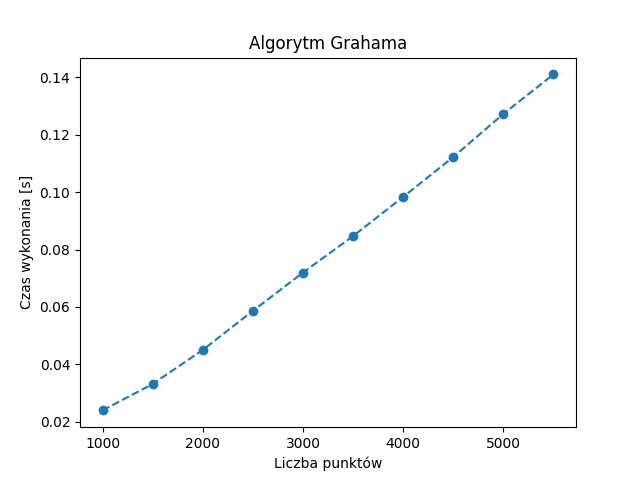
\includegraphics[width=0.95\textwidth]{../tests/chmura-graham.png} % first figure itself
        \caption{Zbiór typu A, algorytm Grahama}
        \label{fig:chmura-graham}
    \end{minipage}\hfill
    \begin{minipage}{0.48\textwidth}
        \centering
        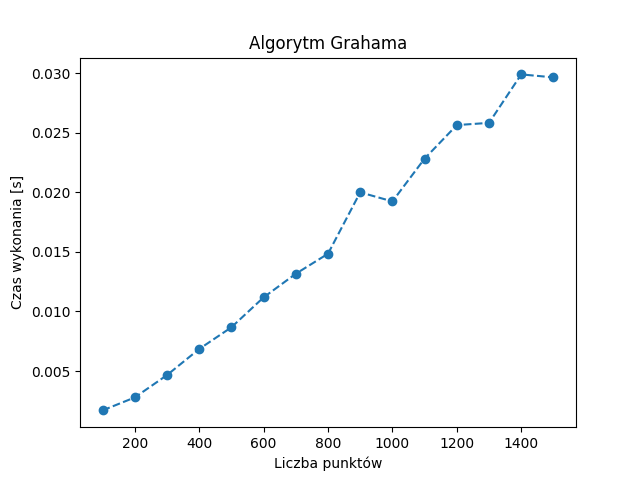
\includegraphics[width=0.95\textwidth]{../tests/okrag-graham.png} % second figure itself
        \caption{Zbiór typu B, algorytm Grahama}
        \label{fig:okrag-graham}
    \end{minipage}
\end{figure}


\begin{figure}[]
    \centering
    \begin{minipage}{0.48\textwidth}
        \centering
        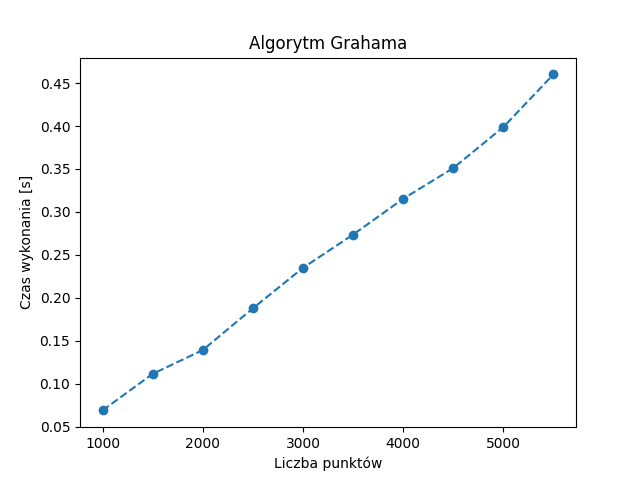
\includegraphics[width=0.95\textwidth]{../tests/prost-graham.png} % first figure itself
        \caption{Zbiór typu C, algorytm Grahama}
        \label{fig:prost-graham}
    \end{minipage}\hfill
    \begin{minipage}{0.48\textwidth}
        \centering
        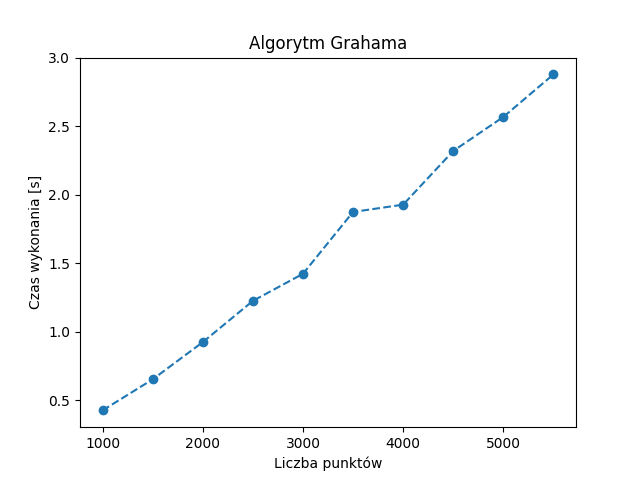
\includegraphics[width=0.95\textwidth]{../tests/kw-graham.png} % second figure itself
        \caption{Zbiór typu D, algorytm Grahama}
        \label{fig:kw-graham}
    \end{minipage}
\end{figure}

\subsection{Algorytm górna-dolna}

W tabeli \ref{tab:lowerupper} przedstawiamy czasy uzyskane przez algorytm górna-dolna dla kolejnych zbiorów punktów, przy różnej liczebności punktów w zbiorze. Na wykresach \ref{fig:chmura-lowerupper}, 
\ref{fig:okrag-lowerupper}, \ref{fig:prost-lowerupper}, \ref{fig:kw-lowerupper} widzimy ilustrację danych z tabeli \ref{tab:lowerupper}.

\begin{table}[]
\centering
\caption{Czas wykonania algorytmu górna-dolna w zależności od typu zbioru testowego oraz mocy zbioru punktów.}
\label{tab:lowerupper}
\begin{tabular}{c|c|c|c|c|c|c|c|c|c|c|}
\cline{2-11}
\multicolumn{1}{l|}{} & \multicolumn{10}{c|}{Liczba punktów} \\ \cline{2-11} 
\multicolumn{1}{l|}{} & 1000 & 1500 & 2000 & 2500 & 3000 & 3500 & 4000 & 4500 & 5000 & 5500 \\ \hline
\multicolumn{1}{|c|}{Typ zbioru} & \multicolumn{10}{c|}{Czas wykonania [s]} \\ \hline
\multicolumn{1}{|c|}{A} & 0.0076 & 0.0079 & 0.0105 & 0.0134 & 0.016 & 0.0186 & 0.0222 & 0.0241 & 0.0269 & 0.0295 \\ \hline
\multicolumn{1}{|c|}{B} & 0.004 & 0.0064 & 0.0086 & 0.0111 & 0.0132 & 0.0164 & 0.018 & 0.0203 & 0.0229 & 0.0254 \\ \hline
\multicolumn{1}{|c|}{C} & 0.0155 & 0.0241 & 0.0321 & 0.0388 & 0.0486 & 0.0549 & 0.0651 & 0.0711 & 0.0784 & 0.084 \\ \hline
\multicolumn{1}{|c|}{D} & 0.0635 & 0.0927 & 0.1261 & 0.1566 & 0.1875 & 0.2217 & 0.259 & 0.2897 & 0.316 & 0.3495 \\ \hline
\end{tabular}
\end{table}

\begin{figure}[]
    \centering
    \begin{minipage}{0.48\textwidth}
        \centering
        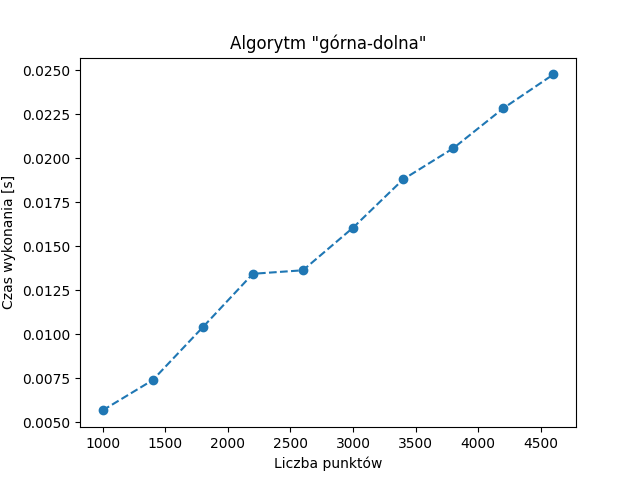
\includegraphics[width=0.95\textwidth]{../tests/chmura-lowerupper.png} % first figure itself
        \caption{Zbiór typu A, algorytm górna-dolna}
        \label{fig:chmura-lowerupper}
    \end{minipage}\hfill
    \begin{minipage}{0.48\textwidth}
        \centering
        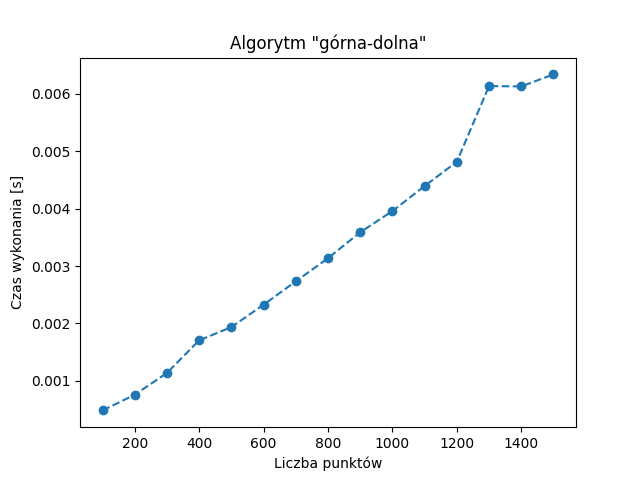
\includegraphics[width=0.95\textwidth]{../tests/okrag-lowerupper.png} % second figure itself
        \caption{Zbiór typu B, algorytm górna-dolna}
        \label{fig:okrag-lowerupper}
    \end{minipage}
\end{figure}


\begin{figure}[]
    \centering
    \begin{minipage}{0.48\textwidth}
        \centering
        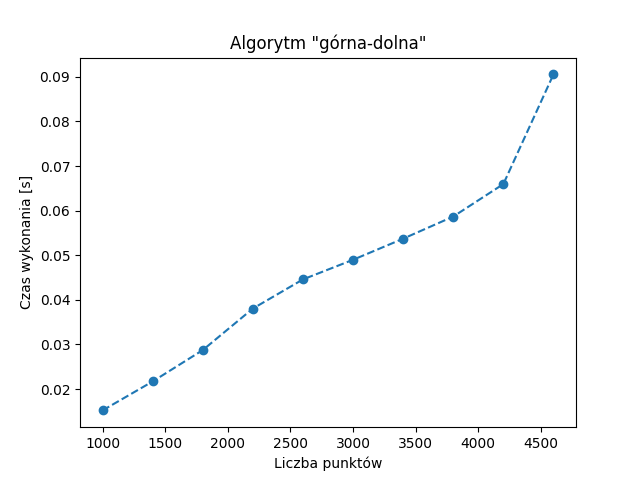
\includegraphics[width=0.95\textwidth]{../tests/prost-lowerupper.png} % first figure itself
        \caption{Zbiór typu C, algorytm górna-dolna}
        \label{fig:prost-lowerupper}
    \end{minipage}\hfill
    \begin{minipage}{0.48\textwidth}
        \centering
        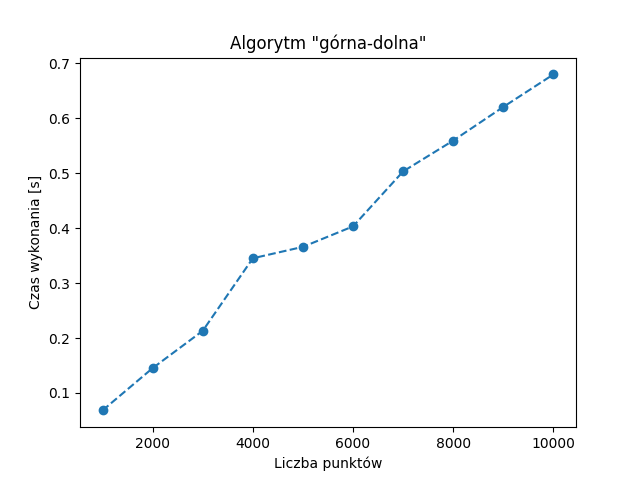
\includegraphics[width=0.95\textwidth]{../tests/kw-lowerupper.png} % second figure itself
        \caption{Zbiór typu D, algorytm górna-dolna}
        \label{fig:kw-lowerupper}
    \end{minipage}
\end{figure}


\subsection{Algorytm Chana}

W tabeli \ref{tab:chan} przedstawiamy czasy uzyskane przez algorytm Chana dla kolejnych zbiorów punktów, przy różnej liczebności punktów w zbiorze. Na wykresach \ref{fig:chmura-chan}, 
\ref{fig:okrag-chan}, \ref{fig:prost-chan}, \ref{fig:kw-chan} widzimy ilustrację danych z tabeli \ref{tab:chan}.

\begin{table}[]
\centering
\caption{Czas wykonania algorytmu Chana w zależności od typu zbioru testowego oraz mocy zbioru punktów.}
\label{tab:chan}
\begin{tabular}{c|c|c|c|c|c|c|c|c|c|c|}
\cline{2-11}
\multicolumn{1}{l|}{} & \multicolumn{10}{c|}{Liczba punktów} \\ \cline{2-11} 
\multicolumn{1}{l|}{} & 1000 & 1500 & 2000 & 2500 & 3000 & 3500 & 4000 & 4500 & 5000 & 5500 \\ \hline
\multicolumn{1}{|c|}{Typ zbioru} & \multicolumn{10}{c|}{Czas wykonania {[}s{]}} \\ \hline
\multicolumn{1}{|c|}{A} & 0.1055 & 0.1544 & 0.3575 & 0.2408 & 0.5449 & 0.6155 & 0.7104 & 0.7904 & 0.8621 & 0.9826 \\ \hline
\multicolumn{1}{|c|}{B} & 0.3714 & 0.5483 & 0.6962 & 0.8893 & 1.0799 & 1.2537 & 1.415 & 1.827 & 1.7746 & 1.9095 \\ \hline
\multicolumn{1}{|c|}{C} & 0.2457 & 0.5615 & 0.727 & 0.9188 & 1.1007 & 1.3044 & 1.5073 & 1.6875 & 1.88 & 2.1234 \\ \hline
\multicolumn{1}{|c|}{D} & 0.6322 & 0.9372 & 1.2306 & 2.1543 & 2.8556 & 6.0844 & 2.4157 & 3.943 & 3.094 & 4.7075 \\ \hline
\end{tabular}
\end{table}

\begin{figure}[]
    \centering
    \begin{minipage}{0.48\textwidth}
        \centering
        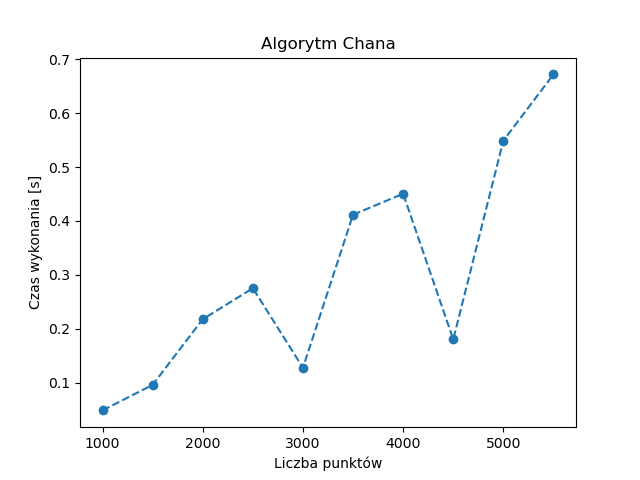
\includegraphics[width=0.95\textwidth]{../tests/chmura-chan.png} % first figure itself
        \caption{Zbiór typu A, algorytm Chana}
        \label{fig:chmura-chan}
    \end{minipage}\hfill
    \begin{minipage}{0.48\textwidth}
        \centering
        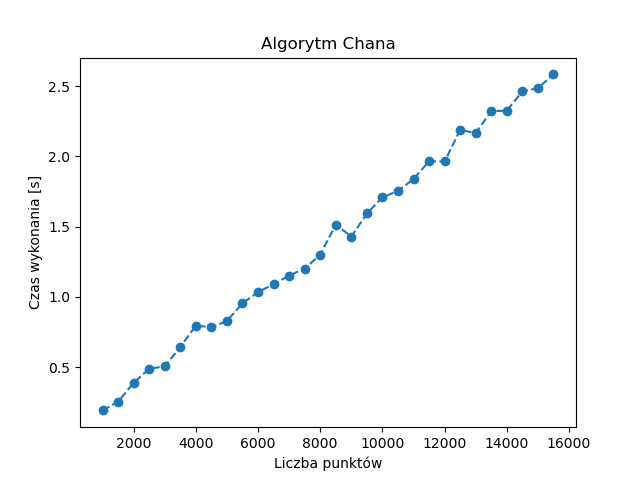
\includegraphics[width=0.95\textwidth]{../tests/okrag-chan.png} % second figure itself
        \caption{Zbiór typu B, algorytm Chana}
        \label{fig:okrag-chan}
    \end{minipage}
\end{figure}

\begin{figure}[]
    \centering
    \begin{minipage}{0.48\textwidth}
        \centering
        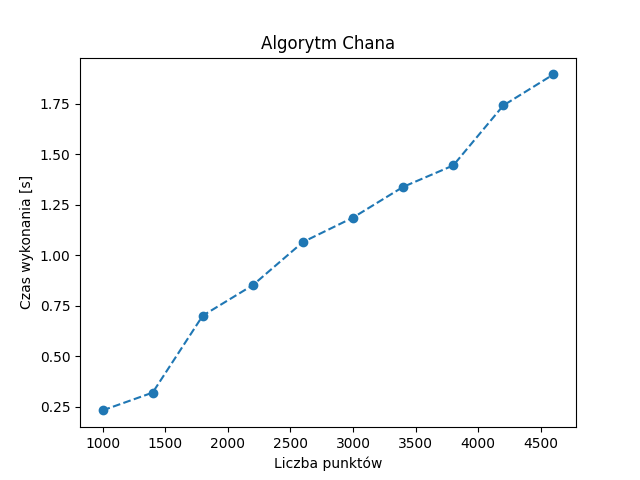
\includegraphics[width=0.95\textwidth]{../tests/prost-chan.png} % first figure itself
        \caption{Zbiór typu C, algorytm Chana}
        \label{fig:prost-chan}
    \end{minipage}\hfill
    \begin{minipage}{0.48\textwidth}
        \centering
        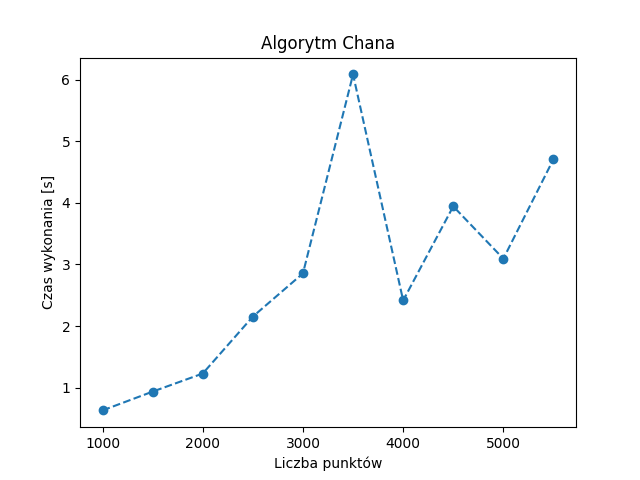
\includegraphics[width=0.95\textwidth]{../tests/kw-chan.png} % second figure itself
        \caption{Zbiór typu D, algorytm Chana}
        \label{fig:kw-chan}
    \end{minipage}
\end{figure}

\subsection{Algorytm QuickHull}

W tabeli \ref{tab:quickhull} przedstawiamy czasy uzyskane przez algorytm QuickHull dla kolejnych zbiorów punktów, przy różnej liczebności punktów w zbiorze. Na wykresach \ref{fig:chmura-quickhull}, 
\ref{fig:okrag-quickhull}, \ref{fig:prost-quickhull}, \ref{fig:kw-quickhull} widzimy ilustrację danych z tabeli \ref{tab:quickhull}.

\begin{table}[]
\centering
\caption{Czas wykonania algorytmu QuickHull w zależności od typu zbioru testowego oraz mocy zbioru punktów.}
\label{tab:quickhull}
\begin{tabular}{c|c|c|c|c|c|c|c|c|c|c|}
\cline{2-11}
\multicolumn{1}{l|}{} & \multicolumn{10}{c|}{Liczba punktów} \\ \cline{2-11} 
\multicolumn{1}{l|}{} & 1000 & 1500 & 2000 & 2500 & 3000 & 3500 & 4000 & 4500 & 5000 & 5500 \\ \hline
\multicolumn{1}{|c|}{Typ zbioru} & \multicolumn{10}{c|}{Czas wykonania {[}s{]}} \\ \hline
\multicolumn{1}{|c|}{A} & 0.0031 & 0.0047 & 0.0058 & 0.0067 & 0.012 & 0.0098 & 0.0134 & 0.0124 & 0.0136 & 0.0155 \\ \hline
\multicolumn{1}{|c|}{B} & 0.0027 & 0.004 & 0.0055 & 0.0082 & 0.0089 & 0.011 & 0.0116 & 0.0133 & 0.0135 & 0.0153 \\ \hline
\multicolumn{1}{|c|}{C} & 0.0064 & 0.0092 & 0.0148 & 0.0153 & 0.0207 & 0.0222 & 0.0256 & 0.0282 & 0.0319 & 0.0348 \\ \hline
\multicolumn{1}{|c|}{D} & 0.0287 & 0.0426 & 0.0551 & 0.0702 & 0.0847 & 0.0986 & 0.1143 & 0.1294 & 0.1411 & 0.1562 \\ \hline
\end{tabular}
\end{table}


\begin{figure}[]
    \centering
    \begin{minipage}{0.48\textwidth}
        \centering
        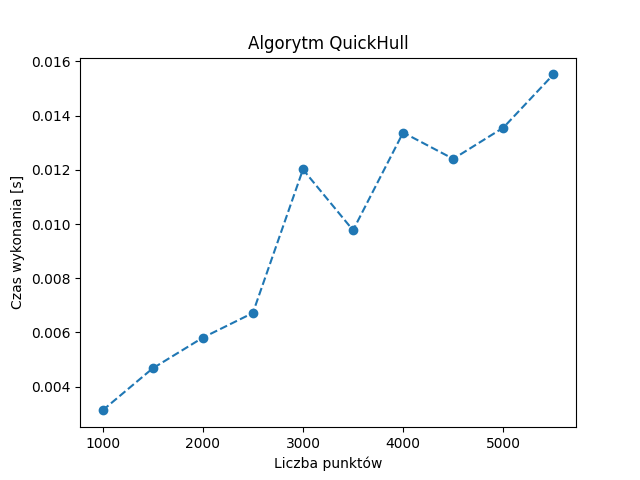
\includegraphics[width=0.95\textwidth]{../tests/chmura-quickhull.png} % first figure itself
        \caption{Zbiór typu A, algorytm QuickHull}
        \label{fig:chmura-quickhull}
    \end{minipage}\hfill
    \begin{minipage}{0.48\textwidth}
        \centering
        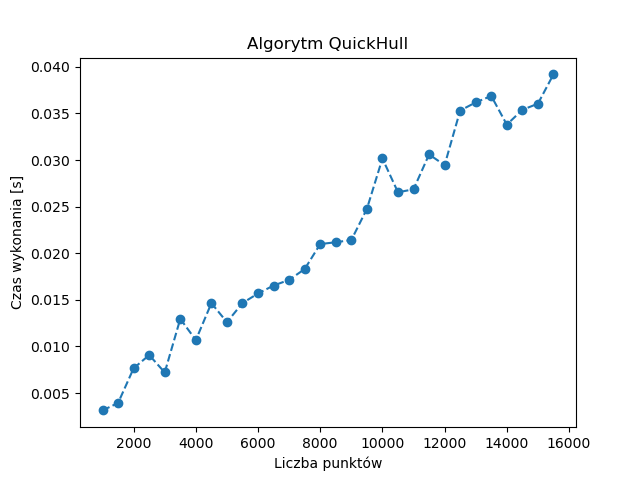
\includegraphics[width=0.95\textwidth]{../tests/okrag-quickhull.png} % second figure itself
        \caption{Zbiór typu B, algorytm QuickHull}
        \label{fig:okrag-quickhull}
    \end{minipage}
\end{figure}



\begin{figure}[]
    \centering
    \begin{minipage}{0.48\textwidth}
        \centering
        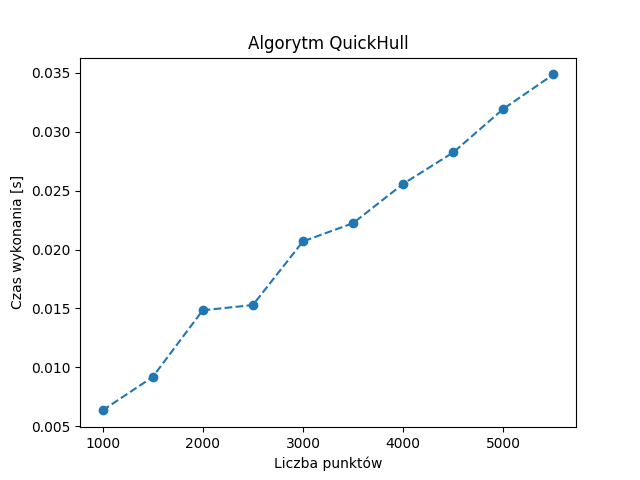
\includegraphics[width=0.95\textwidth]{../tests/prost-quickhull.png} % first figure itself
        \caption{Zbiór typu C, algorytm QuickHull}
        \label{fig:prost-quickhull}
    \end{minipage}\hfill
    \begin{minipage}{0.48\textwidth}
        \centering
        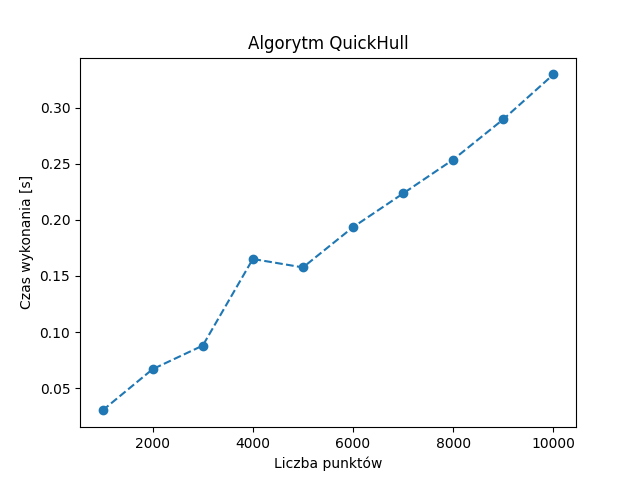
\includegraphics[width=0.95\textwidth]{../tests/kw-quickhull.png} % second figure itself
        \caption{Zbiór typu D, algorytm QuickHull}
        \label{fig:kw-quickhull}
    \end{minipage}
\end{figure}


\subsection{Algorytm dziel i zwyciężaj}

W tabeli \ref{tab:dziel} przedstawiamy czasy uzyskane przez algorytm Dziel i zwyciężaj dla kolejnych zbiorów punktów, przy różnej liczebności punktów w zbiorze. Na wykresach \ref{fig:chmura-dziel}, 
\ref{fig:okrag-dziel}, \ref{fig:prost-dziel}, \ref{fig:kw-dziel} widzimy ilustrację danych z tabeli \ref{tab:dziel}.

\begin{table}[]
\centering
\caption{Czas wykonania algorytmu dziel i zwyciężaj w zależności od typu zbioru testowego oraz mocy zbioru punktów.}
\label{tab:dziel}
\begin{tabular}{c|c|c|c|c|c|c|c|c|c|c|}
\cline{2-11}
\multicolumn{1}{l|}{} & \multicolumn{10}{c|}{Liczba punktów} \\ \cline{2-11} 
\multicolumn{1}{l|}{} & 1000 & 1500 & 2000 & 2500 & 3000 & 3500 & 4000 & 4500 & 5000 & 5500 \\ \hline
\multicolumn{1}{|c|}{Typ zbioru} & \multicolumn{10}{c|}{Czas wykonania {[}s{]}} \\ \hline
\multicolumn{1}{|c|}{A} & 0.0163 & 0.0251 & 0.0341 & 0.0439 & 0.0569 & 0.0631 & 0.0748 & 0.0844 & 0.0955 & 0.1076 \\ \hline
\multicolumn{1}{|c|}{B} & 0.0173 & 0.0234 & 0.0339 & 0.0381 & 0.052 & 0.0562 & 0.0675 & 0.0754 & 0.0829 & 0.0992 \\ \hline
\multicolumn{1}{|c|}{C} & 0.0441 & 0.0683 & 0.0877 & 0.1189 & 0.1516 & 0.1863 & 0.2067 & 0.2437 & 0.27 & 0.3132 \\ \hline
\multicolumn{1}{|c|}{B} & 0.1634 & 0.2474 & 0.3518 & 0.4703 & 0.5694 & 0.6705 & 0.7849 & 0.8928 & 1.0458 & 1.1565 \\ \hline
\end{tabular}
\end{table}

\begin{figure}[]
    \centering
    \begin{minipage}{0.48\textwidth}
        \centering
        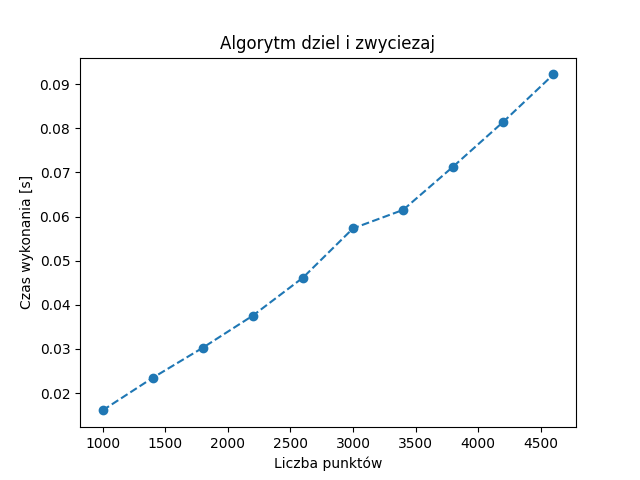
\includegraphics[width=0.95\textwidth]{../tests/chmura-dziel.png} % first figure itself
        \caption{Zbiór typu A, algorytm dziel i zwyciężaj }
        \label{fig:chmura-dziel}
    \end{minipage}\hfill
    \begin{minipage}{0.48\textwidth}
        \centering
        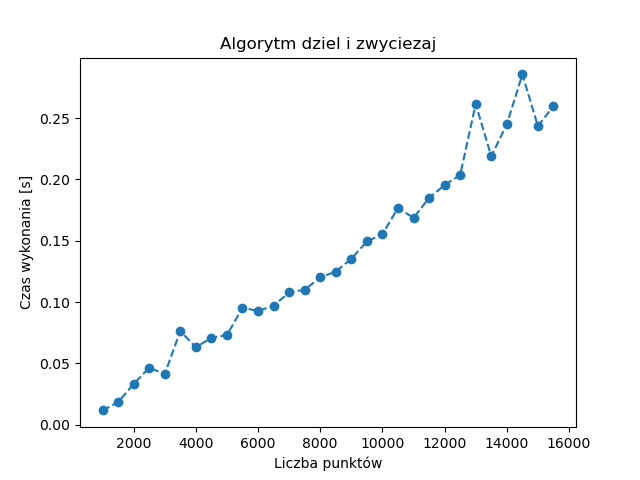
\includegraphics[width=0.95\textwidth]{../tests/okrag-dziel.png} % second figure itself
        \caption{Zbiór typu B, algorytm dziel i zwyciężaj}
        \label{fig:okrag-dziel}
    \end{minipage}
\end{figure}



\begin{figure}[]
    \centering
    \begin{minipage}{0.48\textwidth}
        \centering
        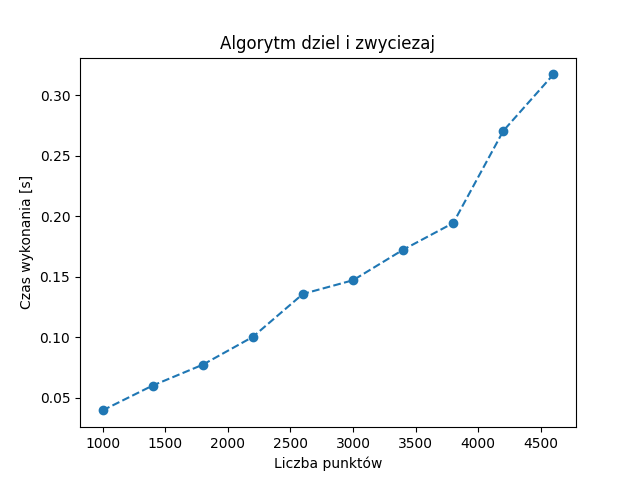
\includegraphics[width=0.95\textwidth]{../tests/prost-dziel.png} % first figure itself
        \caption{Zbiór typu C, algorytm dziel i zwyciężaj}
        \label{fig:prost-dziel}
    \end{minipage}\hfill
    \begin{minipage}{0.48\textwidth}
        \centering
        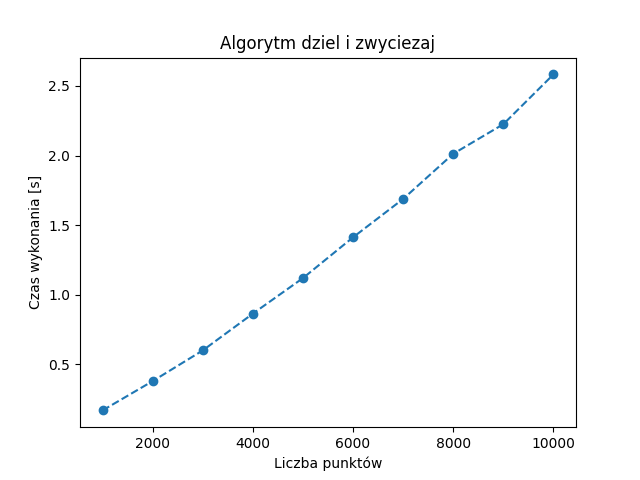
\includegraphics[width=0.95\textwidth]{../tests/kw-dziel.png} % second figure itself
        \caption{Zbiór typu D, algorytm dziel i zwyciężaj}
        \label{fig:kw-dziel}
    \end{minipage}
\end{figure}

\subsection{Algorytm przyrostowy}


W tabeli \ref{tab:przyrost} przedstawiamy czasy uzyskane przez algorytm przyrostowy i zwyciężaj dla kolejnych zbiorów punktów, przy różnej liczebności punktów w zbiorze. Na wykresach \ref{fig:chmura-przyrost}, 
\ref{fig:okrag-przyrost}, \ref{fig:prost-przyrost}, \ref{fig:kw-przyrost} widzimy ilustrację danych z tabeli \ref{tab:przyrost}.

\begin{table}[]
\centering
\caption{Czas wykonania algorytmu przyrostowego w zależności od typu zbioru testowego oraz mocy zbioru punktów.}
\label{tab:przyrost}
\begin{tabular}{c|c|c|c|c|c|c|c|c|c|c|}
\cline{2-11}
\multicolumn{1}{l|}{} & \multicolumn{10}{c|}{Liczba punktów} \\ \cline{2-11} 
\multicolumn{1}{l|}{} & 1000 & 1500 & 2000 & 2500 & 3000 & 3500 & 4000 & 4500 & 5000 & 5500 \\ \hline
\multicolumn{1}{|c|}{Typ zbioru} & \multicolumn{10}{c|}{Czas wykonania {[}s{]}} \\ \hline
\multicolumn{1}{|c|}{A} & 0.0125 & 0.0194 & 0.0251 & 0.0305 & 0.0377 & 0.0431 & 0.0497 & 0.0584 & 0.0621 & 0.0705 \\ \hline
\multicolumn{1}{|c|}{B} & 0.0864 & 0.1788 & 0.2978 & 0.4428 & 0.6359 & 0.7745 & 0.9738 & 1.1858 & 1.3526 & 1.5613 \\ \hline
\multicolumn{1}{|c|}{C} & 0.0315 & 0.0475 & 0.063 & 0.0793 & 0.0997 & 0.1136 & 0.1292 & 0.1449 & 0.1555 & 0.1742 \\ \hline
\multicolumn{1}{|c|}{D} & 0.1373 & 0.1992 & 0.2715 & 0.326 & 0.4165 & 0.4639 & 0.5195 & 0.5937 & 0.6773 & 0.7446 \\ \hline
\end{tabular}
\end{table}

\begin{figure}[]
    \centering
    \begin{minipage}{0.48\textwidth}
        \centering
        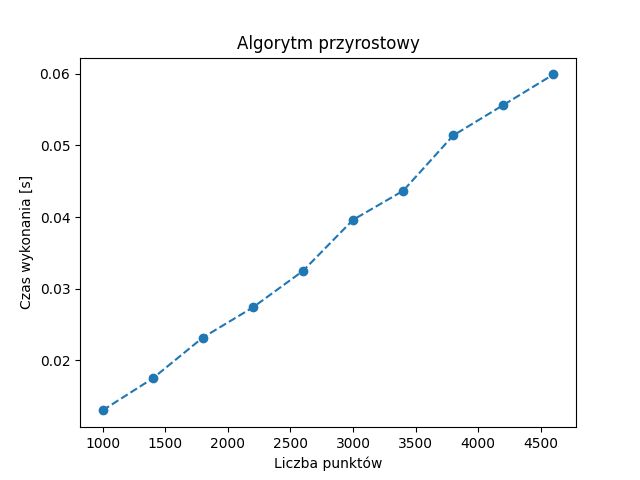
\includegraphics[width=0.95\textwidth]{../tests/chmura-przyrost.png} % first figure itself
        \caption{Zbiór typu A, algorytm przyrostowy}
        \label{fig:chmura-przyrost}
    \end{minipage}\hfill
    \begin{minipage}{0.48\textwidth}
        \centering
        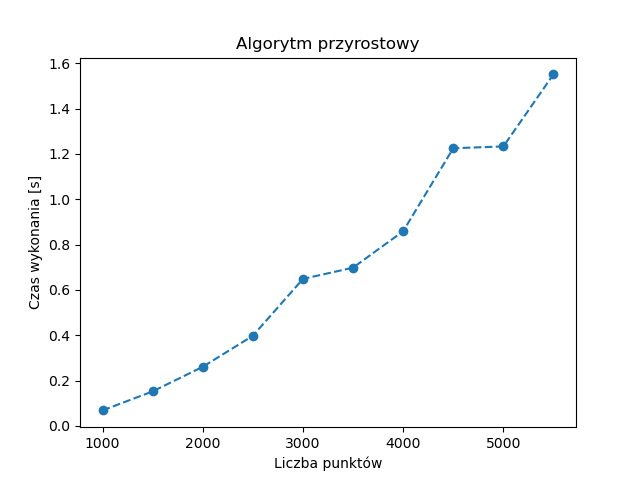
\includegraphics[width=0.95\textwidth]{../tests/okrag-przyrost.png} % second figure itself
        \caption{Zbiór typu B, algorytm przyrostowy}
        \label{fig:okrag-przyrost}
    \end{minipage}
\end{figure}



\begin{figure}[]
    \centering
    \begin{minipage}{0.48\textwidth}
        \centering
        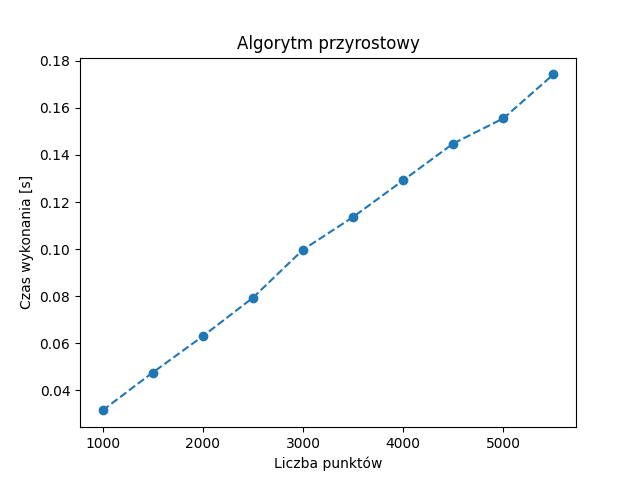
\includegraphics[width=0.95\textwidth]{../tests/prost-przyrost.png} % first figure itself
        \caption{Zbiór typu C, algorytm przyrostowy}
        \label{fig:prost-przyrost}
    \end{minipage}\hfill
    \begin{minipage}{0.48\textwidth}
        \centering
        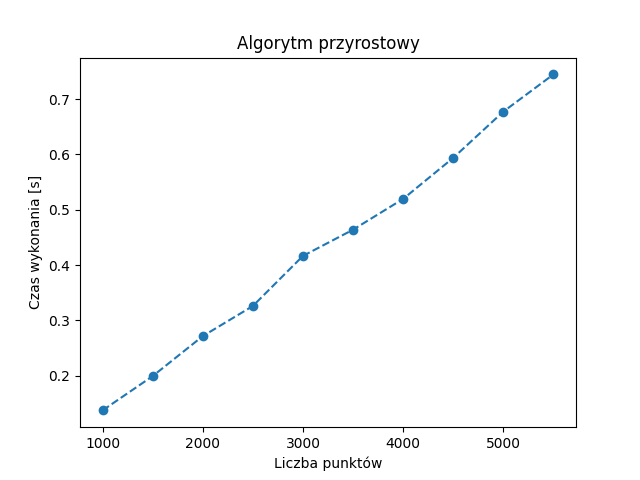
\includegraphics[width=0.95\textwidth]{../tests/kw-przyrost.png} % second figure itself
        \caption{Zbiór typu D, algorytm przyrostowy}
        \label{fig:kw-przyrost}
    \end{minipage}
\end{figure}

\subsection{Algorytm Jarvisa}

W tabeli \ref{tab:jarvis} przedstawiamy czasy uzyskane przez algorytm Jarvisa i zwyciężaj dla kolejnych zbiorów punktów, przy różnej liczebności punktów w zbiorze. Na wykresach \ref{fig:chmura-jarvis}, 
\ref{fig:okrag-jarvis}, \ref{fig:prost-jarvis}, \ref{fig:kw-jarvis} widzimy ilustrację danych z tabeli \ref{tab:jarvis}.

\begin{table}[]
\centering
\caption{Czas wykonania algorytmu Jarvisa w zależności od typu zbioru testowego oraz mocy zbioru punktów.}
\label{tab:jarvis}
\begin{tabular}{c|c|c|c|c|c|c|c|c|c|c|}
\cline{2-11}
\multicolumn{1}{l|}{} & \multicolumn{10}{c|}{Liczba punktów} \\ \cline{2-11} 
\multicolumn{1}{l|}{} & 1000 & 1500 & 2000 & 2500 & 3000 & 3500 & 4000 & 4500 & 5000 & 5500 \\ \hline
\multicolumn{1}{|c|}{Typ danych} & \multicolumn{10}{c|}{Czas wykonania {[}s{]}} \\ \hline
\multicolumn{1}{|c|}{A} & 0.1379 & 0.2058 & 0.2217 & 0.213 & 0.3311 & 0.3635 & 0.307 & 0.3775 & 0.3808 & 0.3825 \\ \hline
\multicolumn{1}{|c|}{B} & 5.684 & 12.882 & 22.737 & 35.648 & 51.305 & 69.425 & 90.227 & 113.80 & 141.27 & 169.58 \\ \hline
\multicolumn{1}{|c|}{C} & 0.0529 & 0.077 & 0.1046 & 0.1306 & 0.1543 & 0.184 & 0.2086 & 0.2304 & 0.2571 & 0.2858 \\ \hline
\multicolumn{1}{|c|}{D} & 0.1094 & 0.1572 & 0.2167 & 0.2611 & 0.3129 & 0.3711 & 0.4218 & 0.4774 & 0.5255 & 0.5886 \\ \hline
\end{tabular}
\end{table}

\begin{figure}[]
    \centering
    \begin{minipage}{0.48\textwidth}
        \centering
        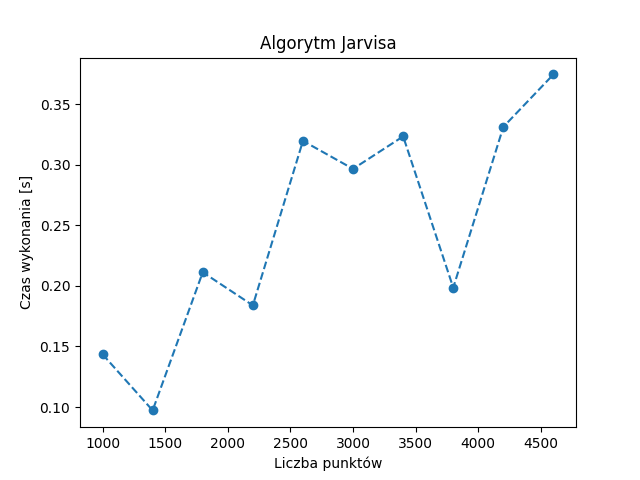
\includegraphics[width=0.95\textwidth]{../tests/chmura-jarvis.png} % first figure itself
        \caption{Zbiór typu A, algorytm Jarvisa}
        \label{fig:chmura-jarvis}
    \end{minipage}\hfill
    \begin{minipage}{0.48\textwidth}
        \centering
        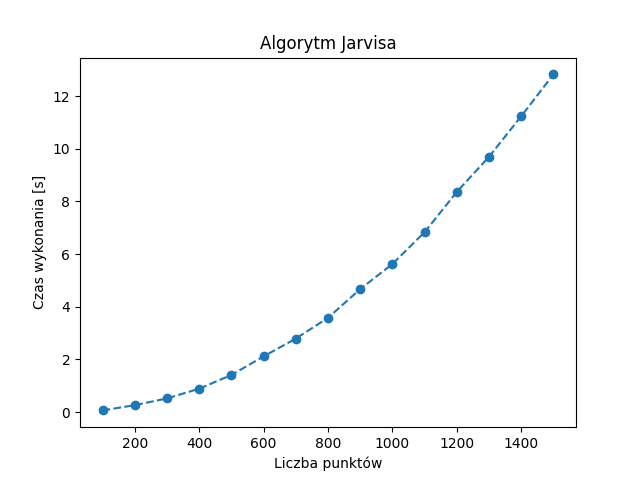
\includegraphics[width=0.95\textwidth]{../tests/okrag-jarvis.png} % second figure itself
        \caption{Zbiór typu B, algorytm Jarvisa}
        \label{fig:okrag-jarvis}
    \end{minipage}
\end{figure}



\begin{figure}[]
    \centering
    \begin{minipage}{0.48\textwidth}
        \centering
        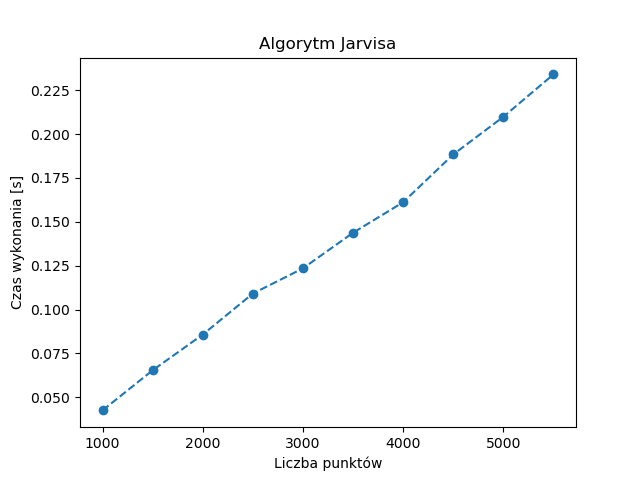
\includegraphics[width=0.95\textwidth]{../tests/prost-jarvis.png} % first figure itself
        \caption{Zbiór typu C, algorytm Jarvisa}
        \label{fig:prost-jarvis}
    \end{minipage}\hfill
    \begin{minipage}{0.48\textwidth}
        \centering
        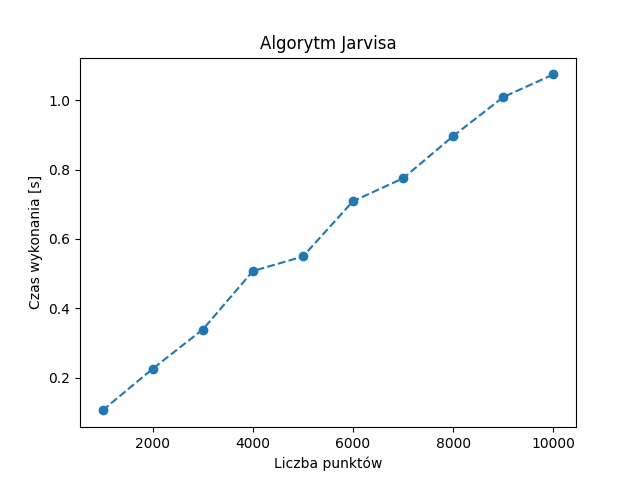
\includegraphics[width=0.95\textwidth]{../tests/kw-jarvis.png} % second figure itself
        \caption{Zbiór typu D, algorytm Jarvisa}
        \label{fig:kw-jarvis}
    \end{minipage}
\end{figure}



\section{Porównanie algorytmów}

Ze względu na różną charakterystykę zbiorów punktów i zachowania algorytmów, porównania dzielimy na 4 sekcje, każda odpowiadająca wybranemu typowi zbioru punktów testowych. 

Dla uproszczenia zapisu w tabelach wprowazdamy oznaczenia dla poszczególnych algorytmów:

\begin{itemize}
    \item $GR$ -- algorytm Grahama
    \item $LU$ -- algorytm górna dolna 
    \item $CH$ -- algorytm Chana
    \item $QH$ -- algorytm QuickHull
    \item $DC$ -- algorytm dziel i zwyciężaj 
    \item $IN$ -- algorytm przyrostowy
    \item $JR$ -- algorytm Jarvisa
\end{itemize}


\subsection{Zbiór typu A}

\begin{table}[]
\centering
\caption{Czasy wykonania poszczególnych algorytmów dla zbioru typu A przy różnych mocach zbiorów punktów.}
\label{tab:chmura}
\begin{tabular}{c|c|c|c|c|c|c|c|c|c|c|}
\cline{2-11}
\multicolumn{1}{l|}{} & \multicolumn{10}{c|}{Liczba punktów} \\ \cline{2-11} 
\multicolumn{1}{l|}{} & 1000 & 1500 & 2000 & 2500 & 3000 & 3500 & 4000 & 4500 & 5000 & 5500 \\ \hline
\multicolumn{1}{|c|}{Algorytm} & \multicolumn{10}{c|}{Czas wykonania {[}s{]}} \\ \hline
\multicolumn{1}{|c|}{$GR$} & 0.0239 & 0.0331 & 0.045 & 0.0586 & 0.072 & 0.0847 & 0.0983 & 0.1122 & 0.1273 & 0.141 \\ \hline
\multicolumn{1}{|c|}{$LU$} & 0.0076 & 0.0079 & 0.0105 & 0.0134 & 0.016 & 0.0186 & 0.0222 & 0.0241 & 0.0269 & 0.0295 \\ \hline
\multicolumn{1}{|c|}{$CH$} & 0.1055 & 0.1544 & 0.3575 & 0.2408 & 0.5449 & 0.6155 & 0.7104 & 0.7904 & 0.8621 & 0.9826 \\ \hline
\multicolumn{1}{|c|}{$QH$} & 0.0031 & 0.0047 & 0.0058 & 0.0067 & 0.012 & 0.0098 & 0.0134 & 0.0124 & 0.0136 & 0.0155 \\ \hline
\multicolumn{1}{|c|}{$DC$} & 0.0163 & 0.0251 & 0.0341 & 0.0439 & 0.0569 & 0.0631 & 0.0748 & 0.0844 & 0.0955 & 0.1076 \\ \hline
\multicolumn{1}{|c|}{$IN$} & 0.0125 & 0.0194 & 0.0251 & 0.0305 & 0.0377 & 0.0431 & 0.0497 & 0.0584 & 0.0621 & 0.0705 \\ \hline
\multicolumn{1}{|c|}{$JR$} & 0.1379 & 0.2058 & 0.2217 & 0.213 & 0.3311 & 0.3635 & 0.307 & 0.3775 & 0.3808 & 0.3825 \\ \hline
\end{tabular}
\end{table}


\begin{figure}[]
    \centering
    \begin{minipage}{0.48\textwidth}
        \centering
        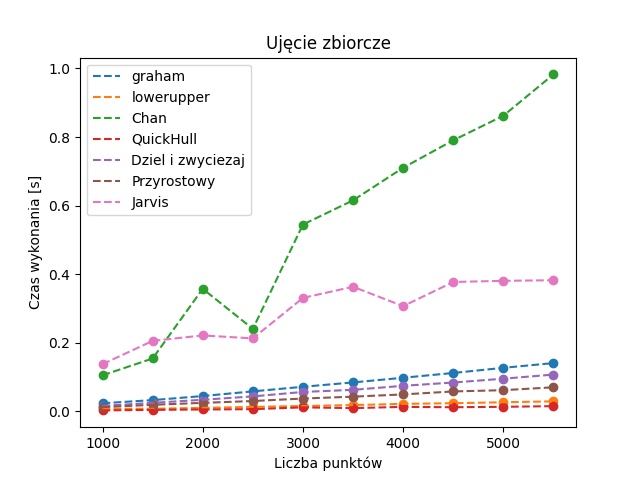
\includegraphics[width=0.95\textwidth]{../tests/chmura-zbiorczy.png} % first figure itself
        \caption{Zbiór typu A, zestawienie}
        \label{fig:chmura-zbiorczy}
    \end{minipage}\hfill
    \begin{minipage}{0.48\textwidth}
        \centering
        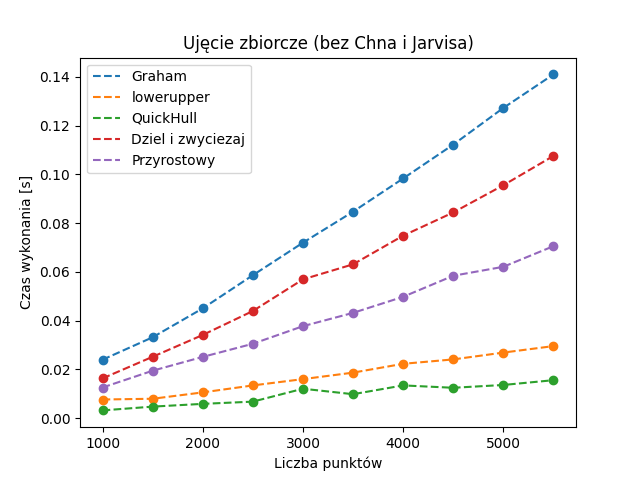
\includegraphics[width=0.95\textwidth]{../tests/chmura-zbiorczy-2.png} % second figure itself
        \caption{Zbiór typu A, zestawienie bez Jarvisa i Chana}
        \label{fig:chmura-zbiorczy-2}
    \end{minipage}
\end{figure}



\subsection{Zbiór typu B}


\begin{table}[]
\centering
\caption{Czasy wykonania poszczególnych algorytmów dla zbioru typu B przy różnych mocach zbiorów punktów. }
\label{tab:okrag}
\begin{tabular}{c|c|c|c|c|c|c|c|c|c|c|}
\cline{2-11}
\multicolumn{1}{l|}{} & \multicolumn{10}{c|}{Liczba punktów} \\ \cline{2-11} 
\multicolumn{1}{l|}{} & 1000 & 1500 & 2000 & 2500 & 3000 & 3500 & 4000 & 4500 & 5000 & 5500 \\ \hline
\multicolumn{1}{|c|}{Algorytm} & \multicolumn{10}{c|}{Czas wykonania {[}s{]}} \\ \hline
\multicolumn{1}{|c|}{$GR$} & 0.0191 & 0.0299 & 0.0413 & 0.0531 & 0.0637 & 0.0768 & 0.0908 & 0.0973 & 0.122 & 0.1284 \\ \hline
\multicolumn{1}{|c|}{$LU$} & 0.004 & 0.0064 & 0.0086 & 0.0111 & 0.0132 & 0.0164 & 0.018 & 0.0203 & 0.0229 & 0.0254 \\ \hline
\multicolumn{1}{|c|}{$CH$} & 0.3714 & 0.5483 & 0.6962 & 0.8893 & 1.0799 & 1.2537 & 1.415 & 1.827 & 1.7746 & 1.9095 \\ \hline
\multicolumn{1}{|c|}{$QH$} & 0.0027 & 0.004 & 0.0055 & 0.0082 & 0.0089 & 0.011 & 0.0116 & 0.0133 & 0.0135 & 0.0153 \\ \hline
\multicolumn{1}{|c|}{$DC$} & 0.0173 & 0.0234 & 0.0339 & 0.0381 & 0.052 & 0.0562 & 0.0675 & 0.0754 & 0.0829 & 0.0992 \\ \hline
\multicolumn{1}{|c|}{$IN$} & 0.0864 & 0.1788 & 0.2978 & 0.4428 & 0.6359 & 0.7745 & 0.9738 & 1.1858 & 1.3526 & 1.5613 \\ \hline
\multicolumn{1}{|c|}{$JR$} & 5.68 & 12.88 & 22.73 & 35.64 & 51.30 & 69.42 & 90.22 & 113.80 & 141.27 & 169.58 \\ \hline
\end{tabular}
\end{table}


\begin{figure}[]
    \centering
    \begin{minipage}{0.48\textwidth}
        \centering
        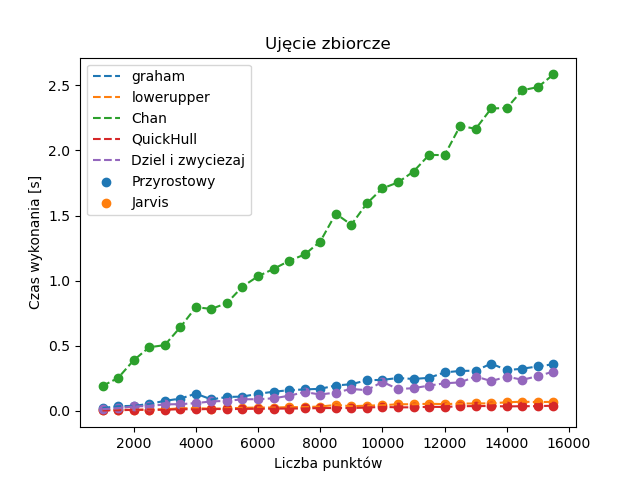
\includegraphics[width=0.95\textwidth]{../tests/okrag-zbiorcze.png} % first figure itself
        \caption{Zbiór typu B, zestawienie}
        \label{fig:okrag-zbiorczy}
    \end{minipage}\hfill
    \begin{minipage}{0.48\textwidth}
        \centering
        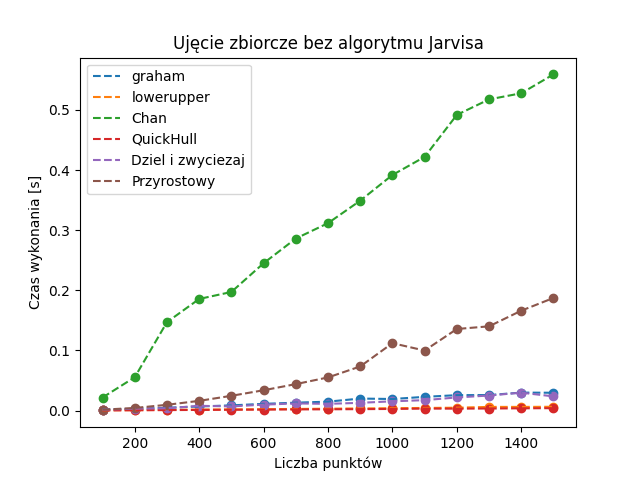
\includegraphics[width=0.95\textwidth]{../tests/okrag-zbiorcze-2.png} % second figure itself
        \caption{Zbiór typu B, zestawienie bez Jarvisa}
        \label{fig:okrag-zbiorczy-2}
    \end{minipage}
\end{figure}


\subsection{Zbiór typu C}

\begin{table}[]
\centering
\caption{Czasy wykonania poszczególnych algorytmów dla zbioru typu C przy różnych mocach zbiorów punktów.}
\label{tab:prost}
\begin{tabular}{c|c|c|c|c|c|c|c|c|c|c|}
\cline{2-11}
\multicolumn{1}{l|}{} & \multicolumn{10}{c|}{Liczba punktów} \\ \cline{2-11} 
\multicolumn{1}{l|}{} & 1000 & 1500 & 2000 & 2500 & 3000 & 3500 & 4000 & 4500 & 5000 & 5500 \\ \hline
\multicolumn{1}{|c|}{Algorytm} & \multicolumn{10}{c|}{Czas wykonania {[}s{]}} \\ \hline
\multicolumn{1}{|c|}{$GR$} & 0.069 & 0.1115 & 0.1392 & 0.1878 & 0.2349 & 0.2736 & 0.3153 & 0.351 & 0.3988 & 0.4601 \\ \hline
\multicolumn{1}{|c|}{$LU$} & 0.0155 & 0.0241 & 0.0321 & 0.0388 & 0.0486 & 0.0549 & 0.0651 & 0.0711 & 0.0784 & 0.084 \\ \hline
\multicolumn{1}{|c|}{$CH$} & 0.2457 & 0.5615 & 0.727 & 0.9188 & 1.1007 & 1.3044 & 1.5073 & 1.6875 & 1.88 & 2.1234 \\ \hline
\multicolumn{1}{|c|}{$QH$} & 0.0064 & 0.0092 & 0.0148 & 0.0153 & 0.0207 & 0.0222 & 0.0256 & 0.0282 & 0.0319 & 0.0348 \\ \hline
\multicolumn{1}{|c|}{$DC$} & 0.0441 & 0.0683 & 0.0877 & 0.1189 & 0.1516 & 0.1863 & 0.2067 & 0.2437 & 0.27 & 0.3132 \\ \hline
\multicolumn{1}{|c|}{$IN$} & 0.0315 & 0.0475 & 0.063 & 0.0793 & 0.0997 & 0.1136 & 0.1292 & 0.1449 & 0.1555 & 0.1742 \\ \hline
\multicolumn{1}{|c|}{$JR$} & 0.0529 & 0.077 & 0.1046 & 0.1306 & 0.1543 & 0.184 & 0.2086 & 0.2304 & 0.2571 & 0.2858 \\ \hline
\end{tabular}
\end{table}

\begin{figure}[]
    \centering
    \begin{minipage}{0.5\textwidth}
        \centering
        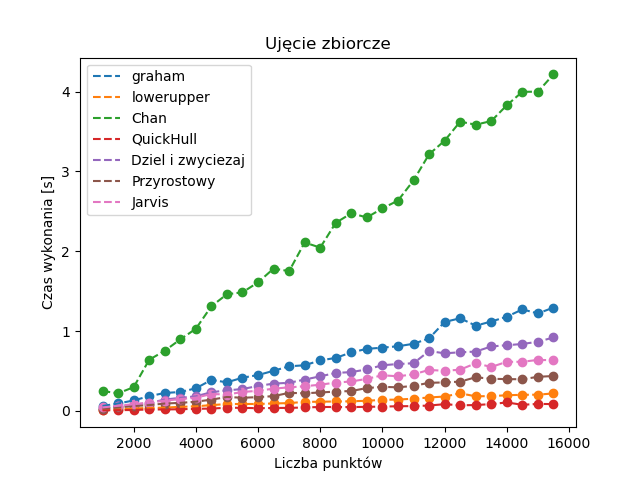
\includegraphics[width=0.95\textwidth]{../tests/prost-zbiorczy.png} % first figure itself
        \caption{Zbiór typu C, zestawienie}
        \label{fig:prost-zbiorczy}
    \end{minipage}\hfill
    \begin{minipage}{0.5\textwidth}
        \centering
        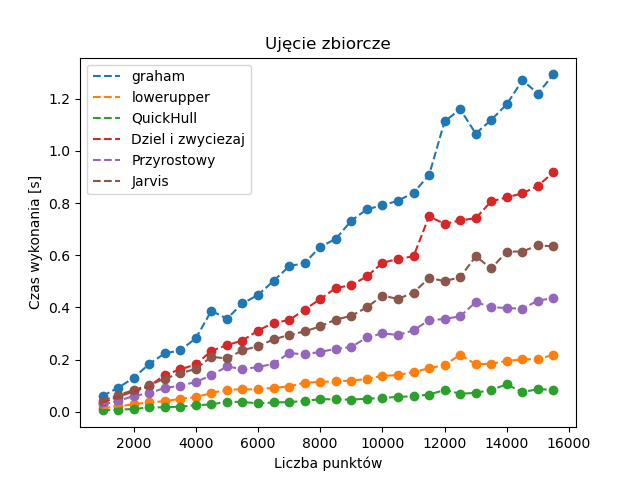
\includegraphics[width=0.95\textwidth]{../tests/prost-zbiorczy-2.png} % second figure itself
        \caption{Zbiór typu C, zestawienie bez Chana}
        \label{fig:prost-zbiorczy-2}
    \end{minipage}
\end{figure}

\subsection{Zbiór typu D}


\begin{table}[]
\centering
\caption{Czasy wykonania poszczególnych algorytmów dla zbioru typu D przy różnych mocach zbiorów punktów.}
\label{tab:kw}
\begin{tabular}{c|c|c|c|c|c|c|c|c|c|c|}
\cline{2-11}
\multicolumn{1}{l|}{} & \multicolumn{10}{c|}{Liczba punktów} \\ \cline{2-11} 
\multicolumn{1}{l|}{} & 1000 & 1500 & 2000 & 2500 & 3000 & 3500 & 4000 & 4500 & 5000 & 5500 \\ \hline
\multicolumn{1}{|c|}{Algorytm} & \multicolumn{10}{c|}{Czas wykonania {[}s{]}} \\ \hline
\multicolumn{1}{|c|}{$GR$} & 0.4256 & 0.6523 & 0.924 & 1.2255 & 1.4233 & 1.8752 & 1.9285 & 2.3207 & 2.5692 & 2.88 \\ \hline
\multicolumn{1}{|c|}{$LU$} & 0.0635 & 0.0927 & 0.1261 & 0.1566 & 0.1875 & 0.2217 & 0.259 & 0.2897 & 0.316 & 0.3495 \\ \hline
\multicolumn{1}{|c|}{$CH$} & 0.6322 & 0.9372 & 1.2306 & 2.1543 & 2.8556 & 6.0844 & 2.4157 & 3.943 & 3.094 & 4.7075 \\ \hline
\multicolumn{1}{|c|}{$QH$} & 0.0287 & 0.0426 & 0.0551 & 0.0702 & 0.0847 & 0.0986 & 0.1143 & 0.1294 & 0.1411 & 0.1562 \\ \hline
\multicolumn{1}{|c|}{$DC$} & 0.1634 & 0.2474 & 0.3518 & 0.4703 & 0.5694 & 0.6705 & 0.7849 & 0.8928 & 1.0458 & 1.1565 \\ \hline
\multicolumn{1}{|c|}{$IN$} & 0.1373 & 0.1992 & 0.2715 & 0.326 & 0.4165 & 0.4639 & 0.5195 & 0.5937 & 0.6773 & 0.7446 \\ \hline
\multicolumn{1}{|c|}{$JR$} & 0.1094 & 0.1572 & 0.2167 & 0.2611 & 0.3129 & 0.3711 & 0.4218 & 0.4774 & 0.5255 & 0.5886 \\ \hline
\end{tabular}
\end{table}

\begin{figure}[]
    \centering
    \begin{minipage}{0.5\textwidth}
        \centering
        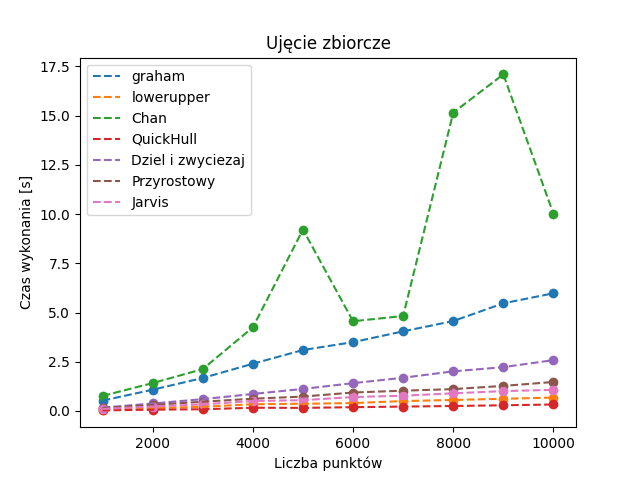
\includegraphics[width=0.95\textwidth]{../tests/kw-zbiorczy.png} % first figure itself
        \caption{Zbiór typu D, zestawienie}
        \label{fig:kw-zbiorczy}
    \end{minipage}\hfill
    \begin{minipage}{0.5\textwidth}
        \centering
        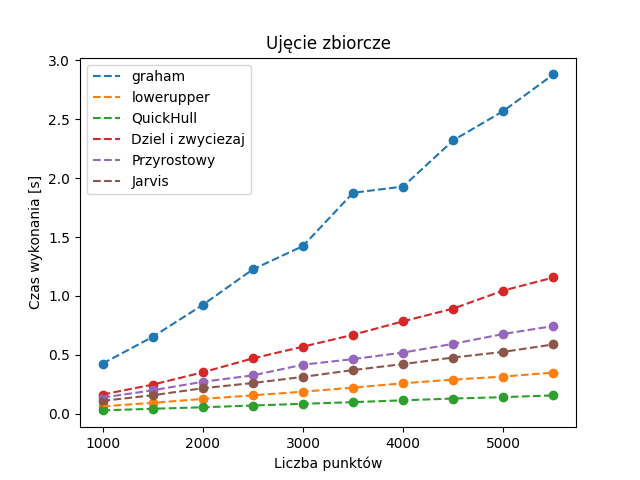
\includegraphics[width=0.95\textwidth]{../tests/kw-zbiorczy-2.png} % second figure itself
        \caption{Zbiór typu D, zestawienie bez Chana}
        \label{fig:kw-zbiorczy-2}
    \end{minipage}
\end{figure}


\section{Bibliografia}

\begin{enumerate}
    \item   \emph{Wykład z przedmiotu Algorytmy Geometryczne, Informatyka 3. sem., 1. st. AGH, Barbara Głut}
    \item   \emph{Computational Geometry -- Algorithms and Applications, Mark de Berg, Otfried Cheong, Marc van Kreveld, Mark Overmars} 
    \item   \begin{verbatim} https://jeffe.cs.illinois.edu/teaching/compgeom/notes/01-convexhull.pdf \end{verbatim}
\end{enumerate}


% \printbibliographyy

\end{document}  